% Options for packages loaded elsewhere
\PassOptionsToPackage{unicode}{hyperref}
\PassOptionsToPackage{hyphens}{url}
\PassOptionsToPackage{dvipsnames,svgnames*,x11names*}{xcolor}
%
\documentclass[
]{krantz}
\usepackage{lmodern}
\usepackage{amssymb,amsmath}
\usepackage{ifxetex,ifluatex}
\ifnum 0\ifxetex 1\fi\ifluatex 1\fi=0 % if pdftex
  \usepackage[T1]{fontenc}
  \usepackage[utf8]{inputenc}
  \usepackage{textcomp} % provide euro and other symbols
\else % if luatex or xetex
  \usepackage{unicode-math}
  \defaultfontfeatures{Scale=MatchLowercase}
  \defaultfontfeatures[\rmfamily]{Ligatures=TeX,Scale=1}
\fi
% Use upquote if available, for straight quotes in verbatim environments
\IfFileExists{upquote.sty}{\usepackage{upquote}}{}
\IfFileExists{microtype.sty}{% use microtype if available
  \usepackage[]{microtype}
  \UseMicrotypeSet[protrusion]{basicmath} % disable protrusion for tt fonts
}{}
\makeatletter
\@ifundefined{KOMAClassName}{% if non-KOMA class
  \IfFileExists{parskip.sty}{%
    \usepackage{parskip}
  }{% else
    \setlength{\parindent}{0pt}
    \setlength{\parskip}{6pt plus 2pt minus 1pt}}
}{% if KOMA class
  \KOMAoptions{parskip=half}}
\makeatother
\usepackage{xcolor}
\IfFileExists{xurl.sty}{\usepackage{xurl}}{} % add URL line breaks if available
\IfFileExists{bookmark.sty}{\usepackage{bookmark}}{\usepackage{hyperref}}
\hypersetup{
  pdftitle={GLMs and Multilevel Models},
  pdfauthor={Paul Roback and Julie Legler},
  colorlinks=true,
  linkcolor=Maroon,
  filecolor=Maroon,
  citecolor=Blue,
  urlcolor=Blue,
  pdfcreator={LaTeX via pandoc}}
\urlstyle{same} % disable monospaced font for URLs
\usepackage{color}
\usepackage{fancyvrb}
\newcommand{\VerbBar}{|}
\newcommand{\VERB}{\Verb[commandchars=\\\{\}]}
\DefineVerbatimEnvironment{Highlighting}{Verbatim}{commandchars=\\\{\}}
% Add ',fontsize=\small' for more characters per line
\usepackage{framed}
\definecolor{shadecolor}{RGB}{248,248,248}
\newenvironment{Shaded}{\begin{snugshade}}{\end{snugshade}}
\newcommand{\AlertTok}[1]{\textcolor[rgb]{0.33,0.33,0.33}{#1}}
\newcommand{\AnnotationTok}[1]{\textcolor[rgb]{0.37,0.37,0.37}{\textbf{\textit{#1}}}}
\newcommand{\AttributeTok}[1]{\textcolor[rgb]{0.61,0.61,0.61}{#1}}
\newcommand{\BaseNTok}[1]{\textcolor[rgb]{0.06,0.06,0.06}{#1}}
\newcommand{\BuiltInTok}[1]{#1}
\newcommand{\CharTok}[1]{\textcolor[rgb]{0.5,0.5,0.5}{#1}}
\newcommand{\CommentTok}[1]{\textcolor[rgb]{0.37,0.37,0.37}{\textit{#1}}}
\newcommand{\CommentVarTok}[1]{\textcolor[rgb]{0.37,0.37,0.37}{\textbf{\textit{#1}}}}
\newcommand{\ConstantTok}[1]{\textcolor[rgb]{0,0,0}{#1}}
\newcommand{\ControlFlowTok}[1]{\textcolor[rgb]{0.27,0.27,0.27}{\textbf{#1}}}
\newcommand{\DataTypeTok}[1]{\textcolor[rgb]{0.27,0.27,0.27}{#1}}
\newcommand{\DecValTok}[1]{\textcolor[rgb]{0.06,0.06,0.06}{#1}}
\newcommand{\DocumentationTok}[1]{\textcolor[rgb]{0.37,0.37,0.37}{\textbf{\textit{#1}}}}
\newcommand{\ErrorTok}[1]{\textcolor[rgb]{0.14,0.14,0.14}{\textbf{#1}}}
\newcommand{\ExtensionTok}[1]{#1}
\newcommand{\FloatTok}[1]{\textcolor[rgb]{0.06,0.06,0.06}{#1}}
\newcommand{\FunctionTok}[1]{\textcolor[rgb]{0,0,0}{#1}}
\newcommand{\ImportTok}[1]{#1}
\newcommand{\InformationTok}[1]{\textcolor[rgb]{0.37,0.37,0.37}{\textbf{\textit{#1}}}}
\newcommand{\KeywordTok}[1]{\textcolor[rgb]{0.27,0.27,0.27}{\textbf{#1}}}
\newcommand{\NormalTok}[1]{#1}
\newcommand{\OperatorTok}[1]{\textcolor[rgb]{0.43,0.43,0.43}{\textbf{#1}}}
\newcommand{\OtherTok}[1]{\textcolor[rgb]{0.37,0.37,0.37}{#1}}
\newcommand{\PreprocessorTok}[1]{\textcolor[rgb]{0.37,0.37,0.37}{\textit{#1}}}
\newcommand{\RegionMarkerTok}[1]{#1}
\newcommand{\SpecialCharTok}[1]{\textcolor[rgb]{0,0,0}{#1}}
\newcommand{\SpecialStringTok}[1]{\textcolor[rgb]{0.5,0.5,0.5}{#1}}
\newcommand{\StringTok}[1]{\textcolor[rgb]{0.5,0.5,0.5}{#1}}
\newcommand{\VariableTok}[1]{\textcolor[rgb]{0,0,0}{#1}}
\newcommand{\VerbatimStringTok}[1]{\textcolor[rgb]{0.5,0.5,0.5}{#1}}
\newcommand{\WarningTok}[1]{\textcolor[rgb]{0.37,0.37,0.37}{\textbf{\textit{#1}}}}
\usepackage{longtable,booktabs}
% Correct order of tables after \paragraph or \subparagraph
\usepackage{etoolbox}
\makeatletter
\patchcmd\longtable{\par}{\if@noskipsec\mbox{}\fi\par}{}{}
\makeatother
% Allow footnotes in longtable head/foot
\IfFileExists{footnotehyper.sty}{\usepackage{footnotehyper}}{\usepackage{footnote}}
\makesavenoteenv{longtable}
\usepackage{graphicx,grffile}
\makeatletter
\def\maxwidth{\ifdim\Gin@nat@width>\linewidth\linewidth\else\Gin@nat@width\fi}
\def\maxheight{\ifdim\Gin@nat@height>\textheight\textheight\else\Gin@nat@height\fi}
\makeatother
% Scale images if necessary, so that they will not overflow the page
% margins by default, and it is still possible to overwrite the defaults
% using explicit options in \includegraphics[width, height, ...]{}
\setkeys{Gin}{width=\maxwidth,height=\maxheight,keepaspectratio}
% Set default figure placement to htbp
\makeatletter
\def\fps@figure{htbp}
\makeatother
\setlength{\emergencystretch}{3em} % prevent overfull lines
\providecommand{\tightlist}{%
  \setlength{\itemsep}{0pt}\setlength{\parskip}{0pt}}
\setcounter{secnumdepth}{5}
\usepackage{booktabs}
%These packages added to resolve tex problems arising from kable tables.
\usepackage{tabularx}
\usepackage{float}
%%
\usepackage{longtable}
\usepackage[bf,singlelinecheck=off]{caption}

\usepackage{framed,color}
\definecolor{shadecolor}{RGB}{248,248,248}

\renewcommand{\textfraction}{0.05}
\renewcommand{\topfraction}{0.8}
\renewcommand{\bottomfraction}{0.8}
\renewcommand{\floatpagefraction}{0.75}

%%%%%%%%
% Inserting new commands here

%% Chapter 2
\newcommand{\lik}{\mathrm{Lik}}
\newcommand{\Lik}{\mathrm{Lik}}

\newcommand{\bstop}{p_{S|B1}}
\newcommand{\nstop}{p_{S|N}}

\newcommand{\thisismynewcommand}{p_{B|\textrm{B Bias}}}
\newcommand{\neutral}{p_{B|N}}
\newcommand{\gbias}{p_{B|\textrm{G Bias}}}
\newcommand{\bbias}{p_{B|\textrm{B Bias}}}

%% Chapter 3
\newcommand{\E}{\operatorname{E}}
\newcommand{\SD}{\operatorname{SD}}

%% Chapter 5
\newcommand{\var}{\operatorname{Var}}

%%%%%%%%

\renewenvironment{quote}{\begin{VF}}{\end{VF}}
\let\oldhref\href
\renewcommand{\href}[2]{#2\footnote{\url{#1}}}

\makeatletter
\newenvironment{kframe}{%
\medskip{}
\setlength{\fboxsep}{.8em}
 \def\at@end@of@kframe{}%
 \ifinner\ifhmode%
  \def\at@end@of@kframe{\end{minipage}}%
  \begin{minipage}{\columnwidth}%
 \fi\fi%
 \def\FrameCommand##1{\hskip\@totalleftmargin \hskip-\fboxsep
 \colorbox{shadecolor}{##1}\hskip-\fboxsep
     % There is no \\@totalrightmargin, so:
     \hskip-\linewidth \hskip-\@totalleftmargin \hskip\columnwidth}%
 \MakeFramed {\advance\hsize-\width
   \@totalleftmargin\z@ \linewidth\hsize
   \@setminipage}}%
 {\par\unskip\endMakeFramed%
 \at@end@of@kframe}
\makeatother

% This change to the shaded environment adapted from https://github.com/yihui/bookdown-chinese/commit/a3e392593b464ba31a7eceb0cd60f7e0bd112798 and https://stackoverflow.com/questions/41052687/rstudio-pdf-knit-fails-with-environment-shaded-undefined-error
\makeatletter
\@ifundefined{Shaded}{
}{\renewenvironment{Shaded}{\begin{kframe}}{\end{kframe}}}
\makeatother

\usepackage{makeidx}
\makeindex

\urlstyle{tt}

\usepackage{amsthm}
\makeatletter
\def\thm@space@setup{%
  \thm@preskip=8pt plus 2pt minus 4pt
  \thm@postskip=\thm@preskip
}
\makeatother

\frontmatter
\usepackage[]{natbib}
\bibliographystyle{plainnat}

\title{GLMs and Multilevel Models}
\usepackage{etoolbox}
\makeatletter
\providecommand{\subtitle}[1]{% add subtitle to \maketitle
  \apptocmd{\@title}{\par {\large #1 \par}}{}{}
}
\makeatother
\subtitle{Broadening Your Statistical Horizons with Applications using R}
\author{Paul Roback and Julie Legler}
\date{2020-06-24}

\begin{document}
\maketitle

% you may need to leave a few empty pages before the dedication page

%\cleardoublepage\newpage\thispagestyle{empty}\null
%\cleardoublepage\newpage\thispagestyle{empty}\null
%\cleardoublepage\newpage
\thispagestyle{empty}

\setlength{\abovedisplayskip}{-5pt}
\setlength{\abovedisplayshortskip}{-5pt}

{
\hypersetup{linkcolor=}
\setcounter{tocdepth}{2}
\tableofcontents
}
\mainmatter

\hypertarget{preface}{%
\chapter*{Preface}\label{preface}}


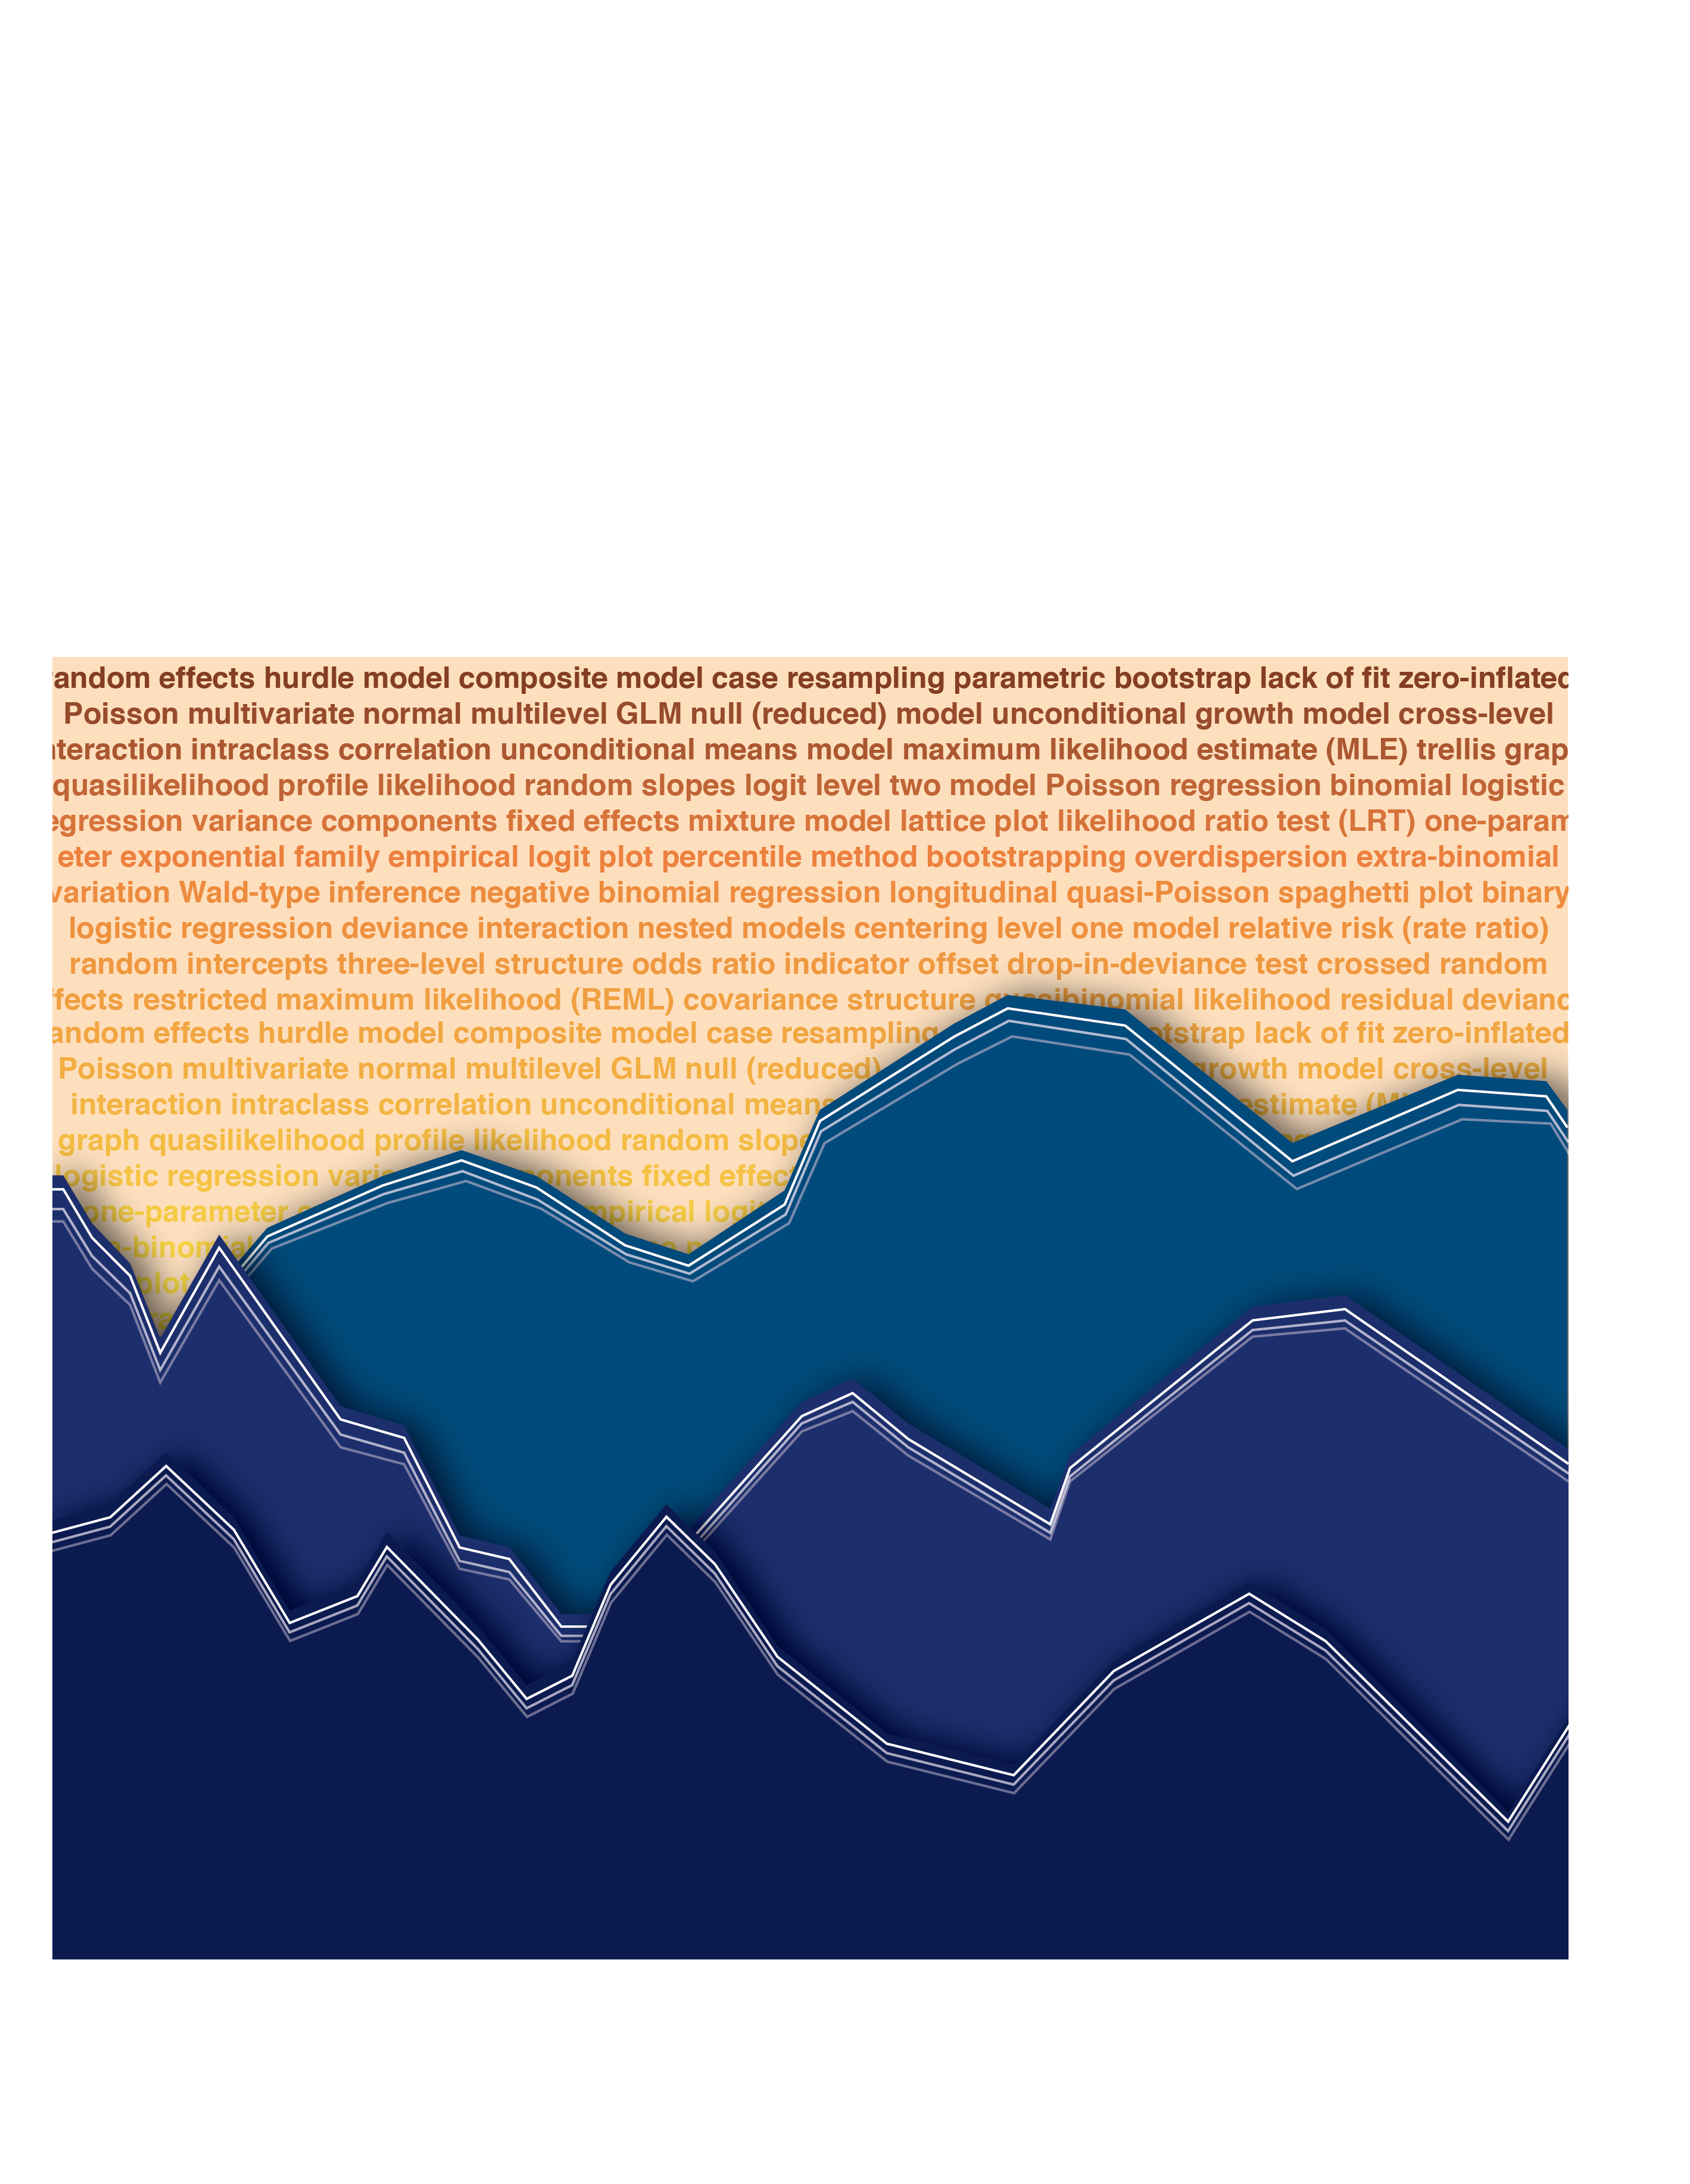
\includegraphics[width=0.75\linewidth]{data/cover}

\textbf{GLMs and Multilevel Models: Broadening Your Statistical Horizons (BYSH) with Applications using R} is intended to be accessible to undergraduate students who have successfully completed a regression course through, for example, a textbook like \emph{Stat2} \citep{Cannon2019}. We started teaching this course at St.~Olaf in 2003 so students would be able to deal with the non-normal, correlated world we live in. It has been offered at St.~Olaf every year since. Even though there is no mathematical prerequisite, we still introduce fairly sophisticated topics such as likelihood theory, zero-inflated Poisson, and parametric bootstrapping in an intuitive and applied manner. We believe strongly in case studies featuring real data and real research questions; thus, most of the data in the textbook and \href{https://github.com/proback/BYSH}{available at our GitHub repo} arises from collaborative research conducted by the authors and their students, or from student projects. Our goal is that, after working through this material, students will not necessarily be expert in these methods and associated theory, but that they will develop an expanded toolkit and a greater appreciation for the wider world of data and statistical modeling.

This work is licensed under a Creative Commons Attribution-NonCommercial-ShareAlike 4.0 International License.

\textbf{Acknowledgements.} We would like to thank students of Stat 316 at St.~Olaf College since 2010 for their patience as this book has taken shape with their feedback. We would especially like to thank these St.~Olaf students for their summer research efforts which significantly improved aspects of this book: Cecilia Noecker, Anna Johanson, Nicole Bettes, Kiegan Rice, Anna Wall, Jack Wolf, Josh Pelayo, Spencer Eanes, and Emily Patterson. Early editions of this book also benefitted greatly from feedback from instructors who used these materials in their classes, including Matt Beckman, Laura Boehm Vock, Beth Chance, Laura Chihara, Mine Dogucu, and Katie Ziegler-Graham. Finally, we have appreciated the support of two NSF grants (\#DMS-1045015 and \#DMS-0354308) and of our colleagues in Mathematics, Statistics, and Computer Science at St.~Olaf.

\hypertarget{ch-multilevelintro}{%
\chapter{Introduction to Multilevel Models}\label{ch-multilevelintro}}

\hypertarget{learning-objectives}{%
\section{Learning Objectives}\label{learning-objectives}}

After finishing this chapter, you should be able to:

\begin{itemize}
\tightlist
\item
  Recognize when response variables and covariates have been collected at multiple (nested) levels.
\item
  Apply exploratory data analysis techniques to multilevel data.
\item
  Write out a multilevel statistical model, including assumptions about variance components, in both by-level and composite forms.
\item
  Interpret model parameters (including fixed effects and variance components) from a multilevel model, including cases in which covariates are continuous, categorical, or centered.
\item
  Understand the taxonomy of models, including why we start with an unconditional means model.
\item
  Select a final model, using criteria such as AIC, BIC, and deviance.
\end{itemize}

\begin{Shaded}
\begin{Highlighting}[]
\CommentTok{# Packages required for Chapter 8}
\KeywordTok{library}\NormalTok{(MASS)}
\KeywordTok{library}\NormalTok{(gridExtra)  }
\KeywordTok{library}\NormalTok{(mnormt) }
\KeywordTok{library}\NormalTok{(lme4) }
\KeywordTok{library}\NormalTok{(knitr) }
\KeywordTok{library}\NormalTok{(tidyverse)}
\end{Highlighting}
\end{Shaded}

\hypertarget{cs:music}{%
\section{Case Study: Music Performance Anxiety}\label{cs:music}}

Stage fright can be a serious problem for performers, and understanding the personality underpinnings of performance anxiety is an important step in determining how to minimize its impact. \citet{Miller2010} studied the emotional state of musicians before performances and factors which may affect their emotional state. Data was collected by having 37 undergraduate music majors from a competitive undergraduate music program fill out diaries prior to performances over the course of an academic year. In particular, study participants completed a Positive Affect Negative Affect Schedule (PANAS) before each performance. The PANAS instrument provided two key outcome measures: negative affect (a state measure of anxiety) and positive affect (a state measure of happiness). We will focus on negative affect as our primary response measuring performance anxiety.

Factors which were examined for their potential relationships with performance anxiety included: performance type (solo, large ensemble, or small ensemble); audience (instructor, public, students, or juried); if the piece was played from memory; age; gender; instrument (voice, orchestral, or keyboard); and, years studying the instrument. In addition, the personalities of study participants were assessed at baseline through the Multidimensional Personality Questionnaire (MPQ). The MPQ provided scores for one lower-order factor (absorption) and three higher-order factors: positive emotionality (PEM---a composite of well-being, social potency, achievement, and social closeness); negative emotionality (NEM---a composite of stress reaction, alienation, and aggression); and, constraint (a composite of control, harm avoidance, and traditionalism).

Primary scientific hypotheses of the researchers included:

\begin{itemize}
\tightlist
\item
  Lower music performance anxiety will be associated with lower levels of a subject's negative emotionality.
\item
  Lower music performance anxiety will be associated with lower levels of a subject's stress reaction.
\item
  Lower music performance anxiety will be associated with greater number of years of study.
\end{itemize}

\hypertarget{explore}{%
\section{Initial Exploratory Analyses}\label{explore}}

\hypertarget{organizedata1}{%
\subsection{Data Organization}\label{organizedata1}}

Our examination of the data from \citet{Miller2010} in \texttt{musicdata.csv} will focus on the following key variables:

\begin{itemize}
\tightlist
\item
  \texttt{id} = unique musician identification number
\item
  \texttt{diary} = cumulative total of diaries filled out by musician
\item
  \texttt{perf\_type} = type of performance (Solo, Large Ensemble, or Small Ensemble)
\item
  \texttt{audience} = who attended (Instructor, Public, Students, or Juried)
\item
  \texttt{memory} = performed from Memory, using Score, or Unspecified
\item
  \texttt{na} = negative affect score from PANAS
\item
  \texttt{gender} = musician gender
\item
  \texttt{instrument} = Voice, Orchestral, or Piano
\item
  \texttt{mpqab} = absorption subscale from MPQ
\item
  \texttt{mpqpem} = positive emotionality (PEM) composite scale from MPQ
\item
  \texttt{mpqnem} = negative emotionality (NEM) composite scale from MPQ
\end{itemize}

Sample rows containing selected variables from our data set are illustrated in Table \ref{tab:table1chp8}; note that each subject (id) has one row for each unique diary entry.

\begin{table}

\caption{\label{tab:table1chp8}A snapshot of selected variables from the first three and the last three observations in the Music Performance Anxiety case study.}
\centering
\resizebox{\linewidth}{!}{
\begin{tabular}[t]{rrrllrllrrr}
\toprule
Obs & id & diary & perf\_type & memory & na & gender & instrument & mpqab & mpqpem & mpqnem\\
\midrule
1 & 1 & 1 & Solo & Unspecified & 11 & Female & voice & 16 & 52 & 16\\
2 & 1 & 2 & Large Ensemble & Memory & 19 & Female & voice & 16 & 52 & 16\\
3 & 1 & 3 & Large Ensemble & Memory & 14 & Female & voice & 16 & 52 & 16\\
495 & 43 & 2 & Solo & Score & 13 & Female & voice & 31 & 64 & 17\\
496 & 43 & 3 & Small Ensemble & Memory & 19 & Female & voice & 31 & 64 & 17\\
\addlinespace
497 & 43 & 4 & Solo & Score & 11 & Female & voice & 31 & 64 & 17\\
\bottomrule
\end{tabular}}
\end{table}

As with any statistical analysis, our first task is to explore the data, examining distributions of individual responses and predictors using graphical and numerical summaries, and beginning to discover relationships between variables. With multilevel models, exploratory analyses must eventually account for the level at which each variable is measured. In a two-level study such as this one, \textbf{Level One} will refer to variables measured at the most frequently occurring observational unit, while \textbf{Level Two} will refer to variables measured on larger observational units. For example, in our study on music performance anxiety, many variables are measured at every performance. These ``Level One'' variables include:

\begin{itemize}
\tightlist
\item
  negative affect (our response variable)
\item
  performance characteristics (type, audience, if music was performed from memory)
\item
  number of previous performances with a diary entry
\end{itemize}

However, other variables measure characteristics of study participants that remain constant over all performances for a particular musician; these are considered ``Level Two'' variables and include:

\begin{itemize}
\tightlist
\item
  demographics (age and gender of musician)
\item
  instrument used and number of previous years spent studying that instrument
\item
  baseline personality assessment (MPQ measures of positive emotionality, negative emotionality, constraint, stress reaction, and absorption)
\end{itemize}

\hypertarget{explore1}{%
\subsection{Exploratory Analyses: Univariate Summaries}\label{explore1}}

Because of this data structure---the assessment of some variables on a performance-by-performance basis and others on a subject-by-subject basis---we cannot treat our data set as consisting of 497 independent observations. Although negative affect measures from different subjects can reasonably be assumed to be independent (unless, perhaps, the subjects frequently perform in the same ensemble group), negative affect measures from different performances by the same subject are not likely to be independent. For example, some subjects tend to have relatively high performance anxiety across all performances, so that knowing their score for Performance 3 was 20 makes it more likely that their score for Performance 5 is somewhere near 20 as well. Thus, we must carefully consider our exploratory data analysis, recognizing that certain plots and summary statistics may be useful but imperfect in light of the correlated observations.

First, we will examine each response variable and potential covariate individually. Continuous variables can be summarized using histograms and summaries of center and spread; categorical variables can be summarized with tables and possibly bar charts. When examining Level One covariates and responses, we will begin by considering all 497 observations, essentially treating each performance by each subject as independent even though we expect observations from the same musician to be correlated. Although these plots will contain dependent points, since each musician provides data for up to 15 performances, general patterns exhibited in these plots tend to be real. Alternatively, we can calculate mean scores across all performances for each of the 37 musicians so that we can more easily consider each plotted point to be independent. The disadvantage of this approach would be lost information which, in a study such as this with a relatively small number of musicians each being observed over many performances, could be considerable. In addition, if the sample sizes varied greatly by subject, a mean based on 1 observation would be given equal weight to a mean based on 15 observations. Nevertheless, both types of exploratory plots typically illustrate similar relationships.

In Figure \ref{fig:mli-hist1} we see histograms for the primary response (negative affect); plot (a) shows all 497 (dependent) observations, while plot (b) shows the mean negative affect for each of the 37 musicians across all their performances. Through plot (a), we see that performance anxiety (negative affect) across all performances follows a right skewed distribution with a lower bound of 10 (achieved when all 10 questions are answered with a 1). Plot (b) shows that mean negative affect is also right-skewed (although not as smoothly decreasing in frequency), with range 12 to 23.

\begin{figure}

{\centering 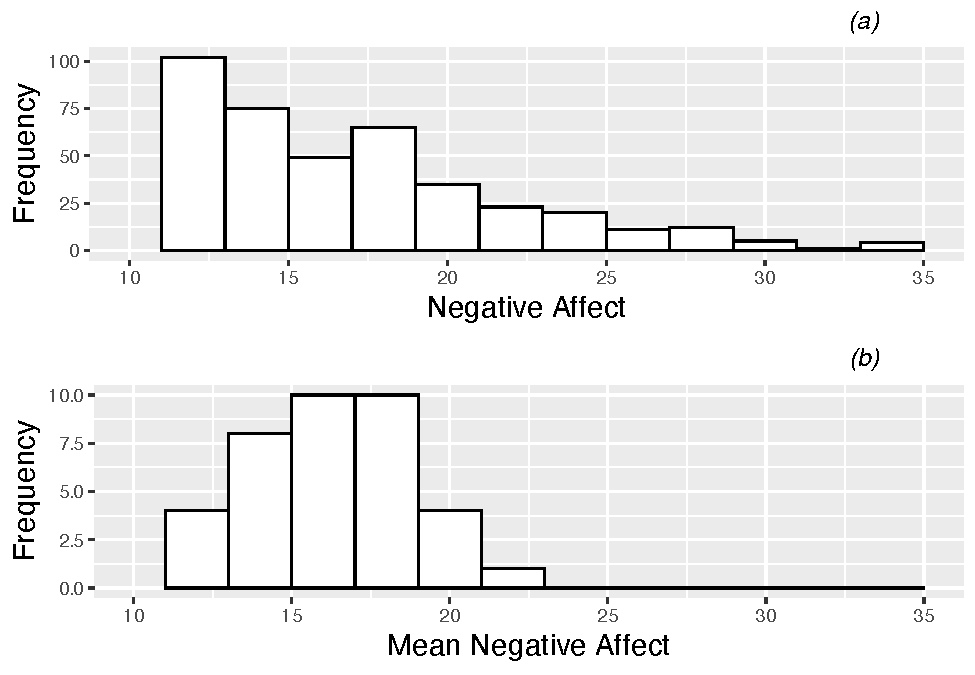
\includegraphics[width=0.6\linewidth]{bookdown-bysh_files/figure-latex/mli-hist1-1} 

}

\caption{Histogram of the continuous Level One response (negative effect). Plot (a) contains all 497 performances across the 37 musicians, while plot (b) contains one observation per musician (the mean negative affect across all performances).}\label{fig:mli-hist1}
\end{figure}

We can also summarize categorical Level One covariates across all (possibly correlated) observations to get a rough relative comparison of trends. 56.1\% of the 497 performances in our data set were solos, while 27.3\% were large ensembles and 16.5\% were small ensembles. The most common audience type was a public performance (41.0\%), followed by instructors (30.0\%), students (20.1\%), and finally juried recitals (8.9\%). In 30.0\% of performances, the musician played by memory, while 55.1\% used the score and 14.9\% of performances were unspecified.

To generate an initial examination of Level Two covariates, we consider a data set with just one observation per subject, since Level Two variables are constant over all performances from the same subject. Then, we can proceed as we did with Level One covariates---using histograms to illustrate the distributions of continuous covariates (see Figure \ref{fig:mli-histmat1}) and tables to summarize categorical covariates. For example, we learn that the majority of subjects have positive emotionality scores between 50 and 60, but that several subjects fall into a lengthy lower tail with scores between 20 and 50. A summary of categorical Level Two covariates reveals that among the 37 subjects (26 female and 11 male), 17 play an orchestral instrument, 15 are vocal performers, and 5 play a keyboard instrument.

\begin{figure}

{\centering 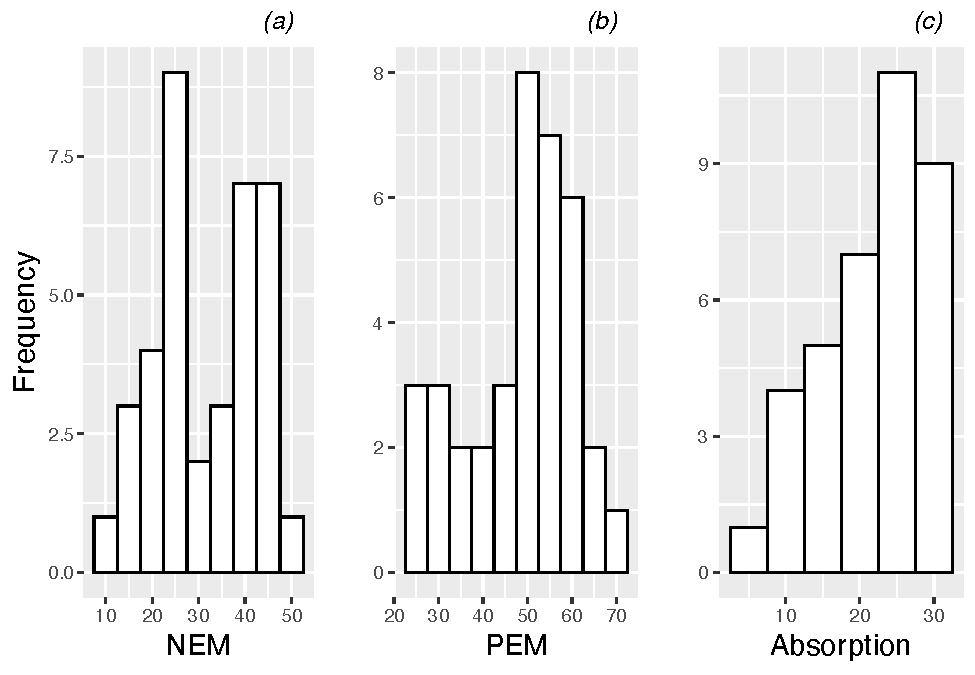
\includegraphics[width=0.6\linewidth]{bookdown-bysh_files/figure-latex/mli-histmat1-1} 

}

\caption{Histograms of the 3 continuous Level Two covariates (negative emotionality (NEM), positive emotionality (PEM), and absorption).  Each plot contains one observation per musician.}\label{fig:mli-histmat1}
\end{figure}

\hypertarget{explore2}{%
\subsection{Exploratory Analyses: Bivariate Summaries}\label{explore2}}

The next step in an initial exploratory analysis is the examination of numerical and graphical summaries of relationships between model covariates and responses. In examining these bivariate relationships, we hope to learn: (1) if there is a general trend suggesting that as the covariate increases the response either increases or decreases, (2) if subjects at certain levels of the covariate tend to have similar mean responses (low variability), and (3) if the variation in the response differs at different levels of the covariate (unequal variability).

As with individual variables, we will begin by treating all 497 performances recorded as independent observations, even though blocks of 15 or so performances were performed by the same musician. For categorical Level One covariates, we can generate boxplots against negative affect as in Figure \ref{fig:mli-boxscatmat1}, plots (a) and (b). From these boxplots, we see that lower levels of performance anxiety seem to be associated with playing in large ensembles and playing in front of an instructor. For our lone continuous Level One covariate (number of previous performances), we can generate a scatterplot against negative affect as in plot (c) from Figure \ref{fig:mli-boxscatmat1}, adding a fitted line to illustrate general trends upward or downward. From this scatterplot, we see that negative affect seems to decrease slightly as a subject has more experience.

To avoid the issue of dependent observations in our three plots from Figure \ref{fig:mli-boxscatmat1}, we could generate separate plots for each subject and examine trends within and across subjects. These ``lattice plots'' are illustrated in Figures \ref{fig:mli-lattice1}, \ref{fig:mli-lattice2}, and \ref{fig:mli-lattice3}; we discuss such plots more thoroughly in Chapter \ref{ch-lon}. While general trends are difficult to discern from these lattice plots, we can see the variety in subjects in sample size distributions and overall level of performance anxiety. In particular, in Figure \ref{fig:mli-lattice3}, we notice that linear fits for many subjects illustrate the same same slight downward trend displayed in the overall scatterplot in Figure \ref{fig:mli-boxscatmat1}, although some subjects experience increasing anxiety and others exhibit non-linear trends. Having an idea of the range of individual trends will be important when we begin to draw overall conclusions from this study.

\begin{figure}

{\centering 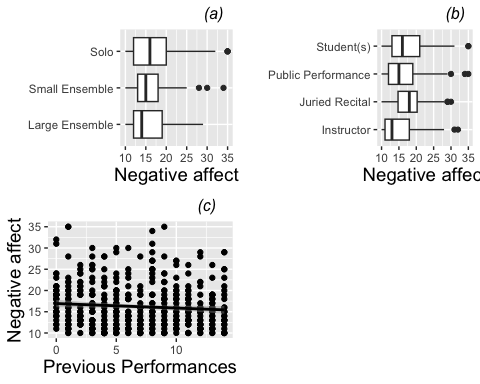
\includegraphics[width=0.6\linewidth]{bookdown-bysh_files/figure-latex/mli-boxscatmat1-1} 

}

\caption{Boxplots of two categorical Level One covariates (performance type (a) and audience type (b)) vs. model response, and scatterplot of one continuous Level One covariate (number of previous diary entries (c)) vs. model response (negative affect).  Each plot contains one observation for each of the 497 performances.}\label{fig:mli-boxscatmat1}
\end{figure}

\begin{figure}

{\centering 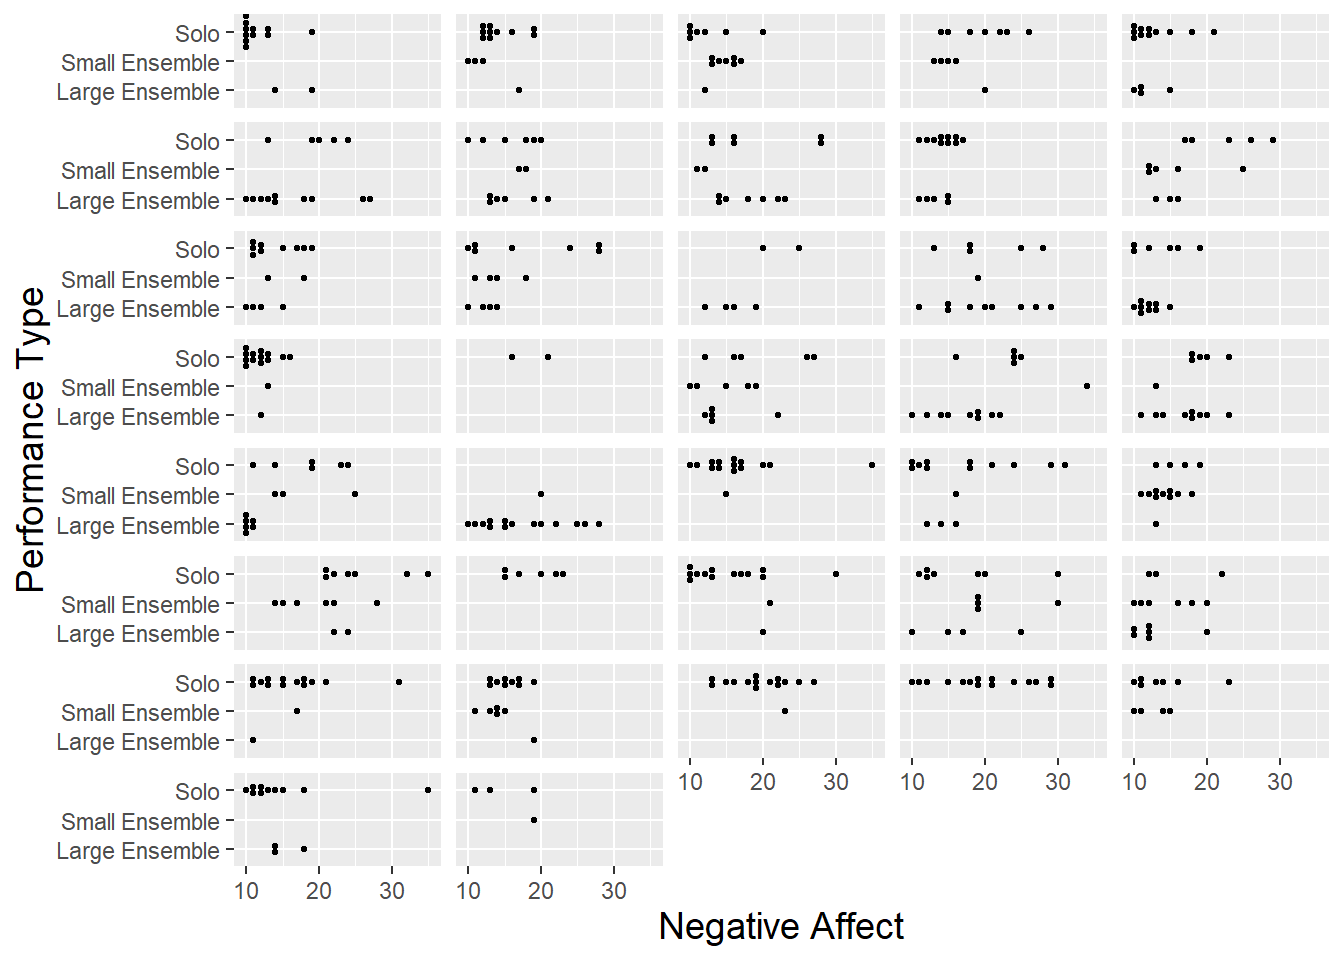
\includegraphics[width=0.6\linewidth]{bookdown-bysh_files/figure-latex/mli-lattice1-1} 

}

\caption{Lattice plot of performance type vs. negative affect, with separate dotplots by subject.}\label{fig:mli-lattice1}
\end{figure}

\begin{figure}

{\centering 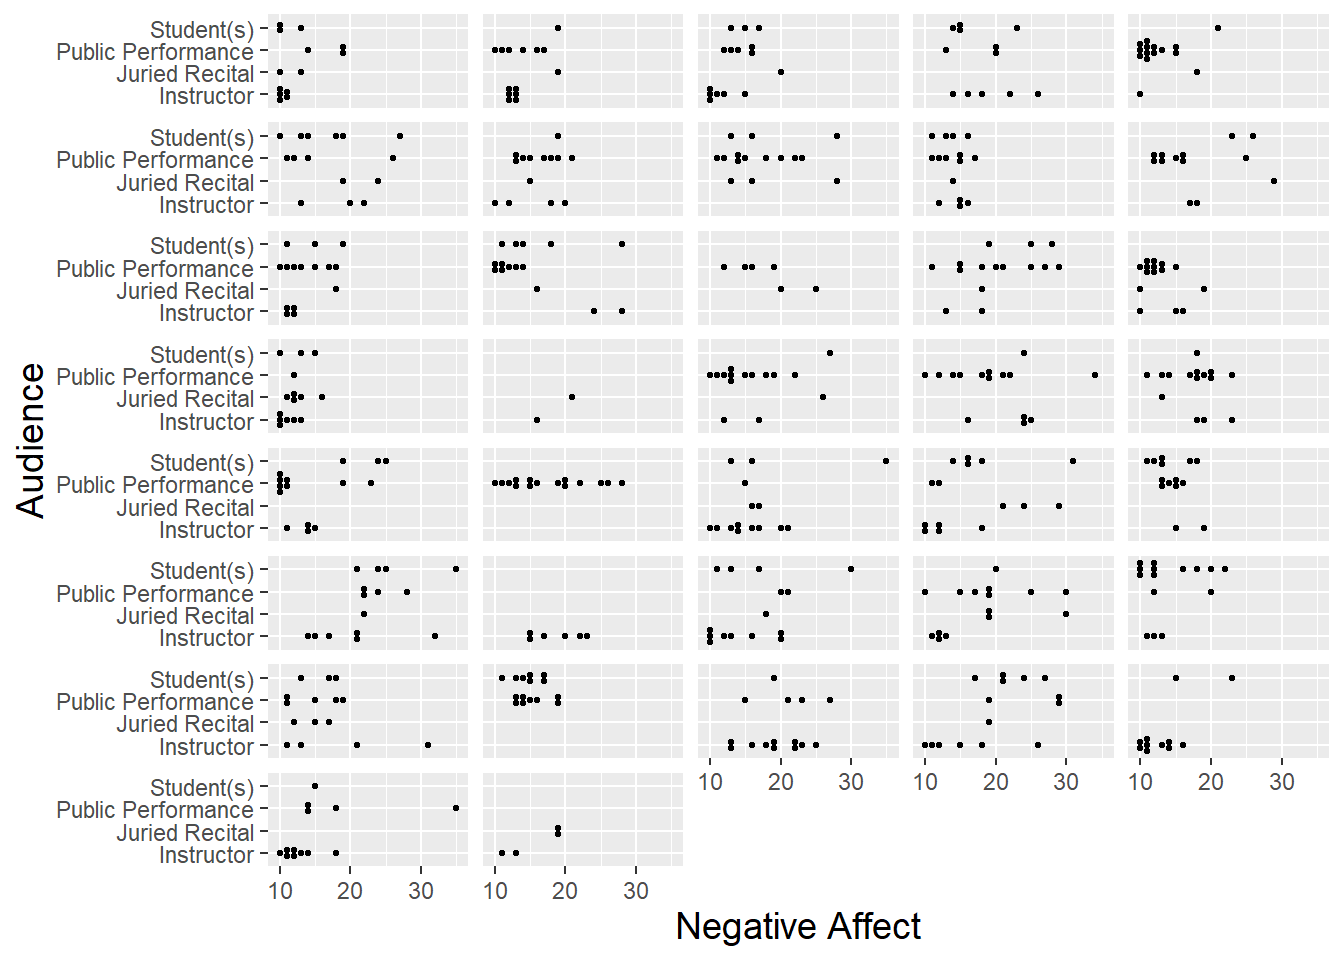
\includegraphics[width=0.6\linewidth]{bookdown-bysh_files/figure-latex/mli-lattice2-1} 

}

\caption{Lattice plot of audience type vs. negative affect, with separate dotplots by subject.}\label{fig:mli-lattice2}
\end{figure}

\begin{figure}

{\centering 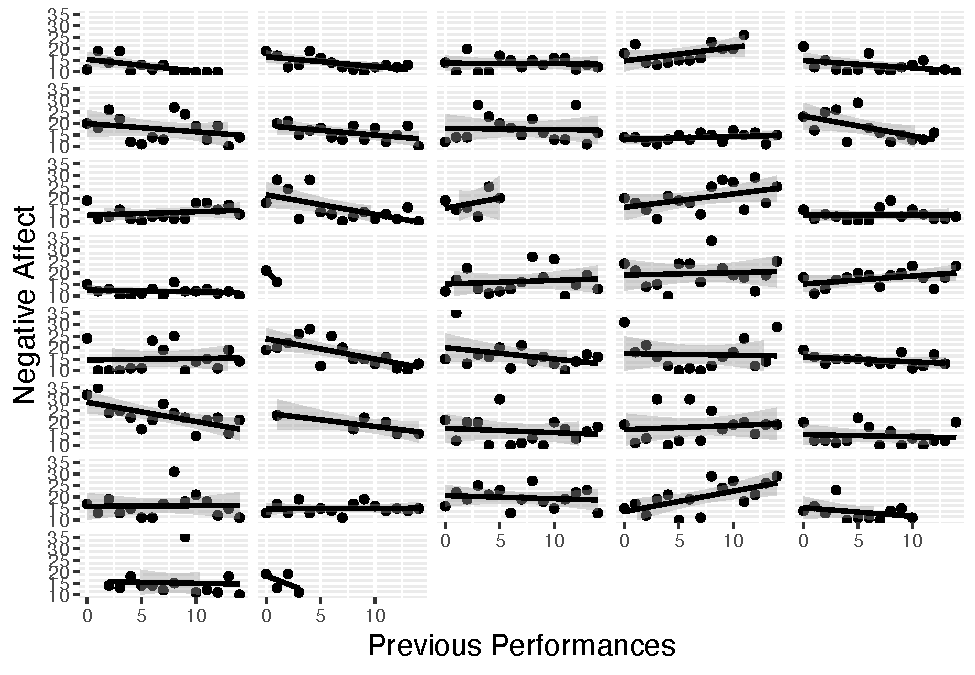
\includegraphics[width=0.6\linewidth]{bookdown-bysh_files/figure-latex/mli-lattice3-1} 

}

\caption{Lattice plot of previous performances vs. negative affect, with separate scatterplots with fitted lines by subject.}\label{fig:mli-lattice3}
\end{figure}

In Figure \ref{fig:mli-boxmat1}, we use boxplots to examine the relationship between our primary categorical Level Two covariate (instrument) and our continuous model response. Plot (a) uses all 497 performances, while plot (b) uses one observation per subject (the mean performance anxiety across all performances) regardless of how many performances that subject had. Naturally, plot (b) has a more condensed range of values, but both plots seem to support the notion that performance anxiety is slightly lower for vocalists and maybe a bit higher for keyboardists

\begin{figure}

{\centering 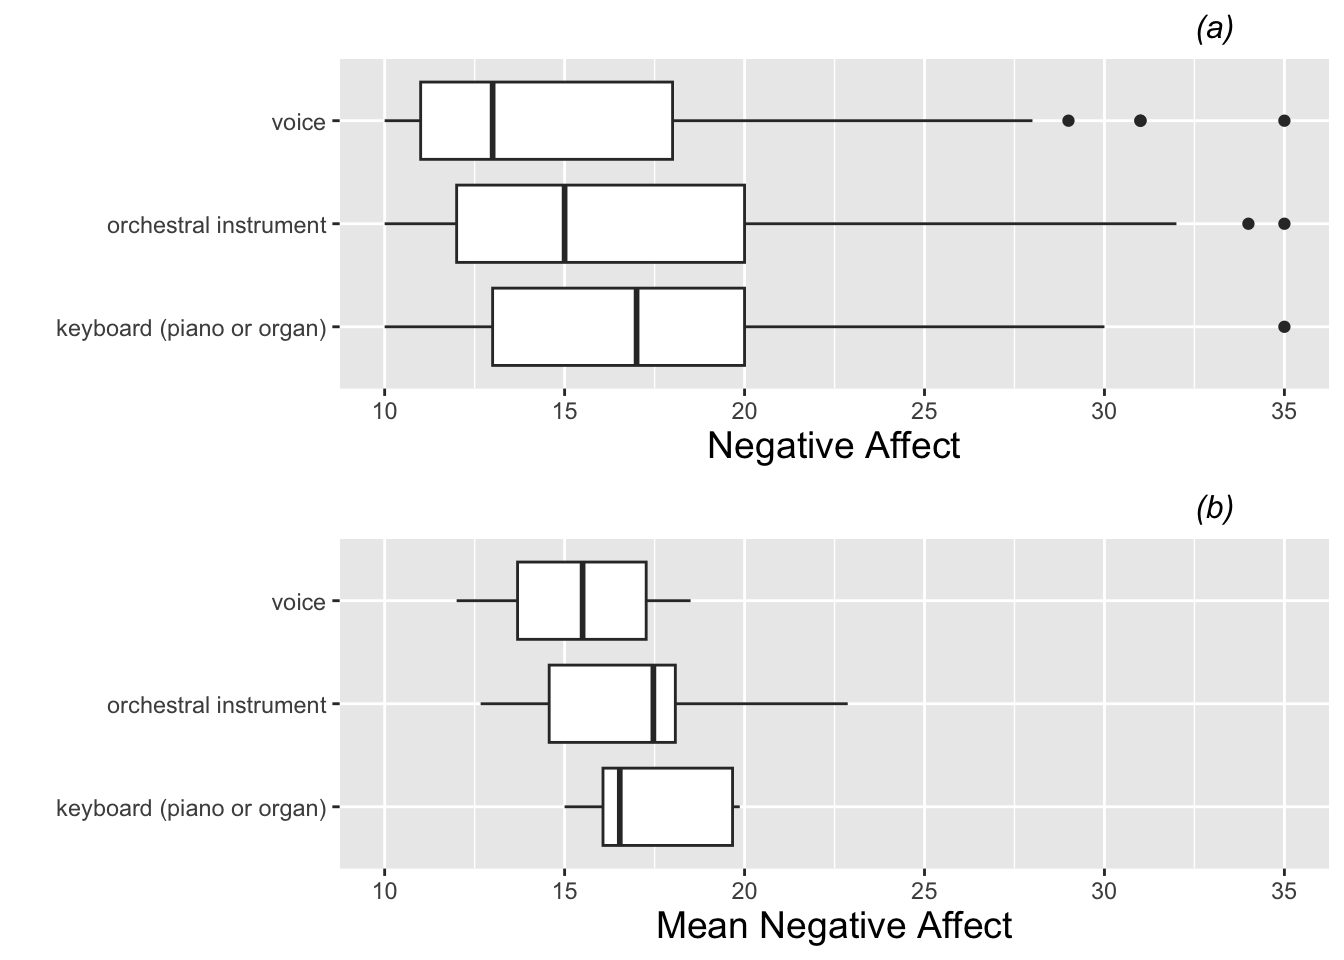
\includegraphics[width=0.6\linewidth]{bookdown-bysh_files/figure-latex/mli-boxmat1-1} 

}

\caption{Boxplots of the categorical Level Two covariate (instrument) vs. model response (negative affect).  Plot (a) is based on all 497 observations from all 37 subjects, while plot (b) uses only one observation per subject.}\label{fig:mli-boxmat1}
\end{figure}

In Figure \ref{fig:mli-scatmat1}, we use scatterplots to examine the relationships between continuous Level Two covariates and our model response. Performance anxiety appears to vary little with a subject's positive emotionality, but there is some evidence to suggest that performance anxiety increases with increasing negative emotionality and absorption level. Plots based on mean negative affect, with one observation per subject, support conclusions based on plots with all observations from all subjects; indeed the overall relationships are in the same direction and of the same magnitude.

\begin{figure}

{\centering 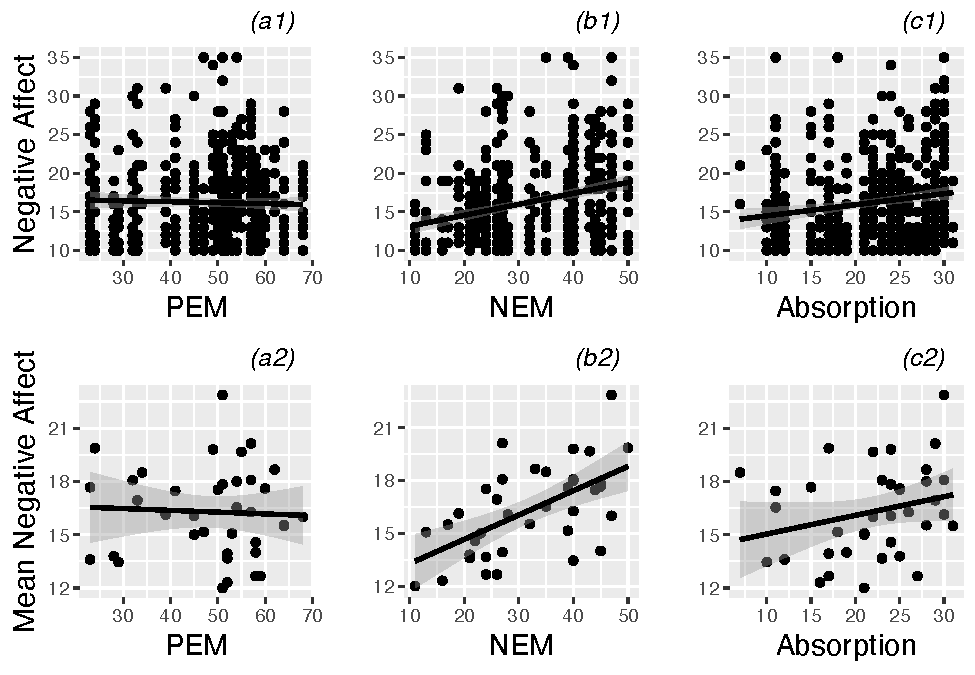
\includegraphics[width=0.6\linewidth]{bookdown-bysh_files/figure-latex/mli-scatmat1-1} 

}

\caption{ Scatterplots of continuous Level Two covariates (positive emotionality (PEM), negative emotionality (NEM), and absorption) vs. model response (negative affect).  The top plots (a1, b1, c1) are based on all 497 observations from all 37 subjects, while the bottom plots (a2, b2, c2) use only one observation per subject.}\label{fig:mli-scatmat1}
\end{figure}

Of course, any graphical analysis is exploratory, and any notable trends at this stage should be checked through formal modeling. At this point, a statistician begins to ask familiar questions such as:

\begin{itemize}
\tightlist
\item
  which characteristics of individual performances are most associated with performance anxiety?
\item
  which characteristics of study participants are most associated with performance anxiety?
\item
  are any of these associations statistically significant?
\item
  does the significance remain after controlling for other covariates?
\item
  how do we account for the lack of independence in performances by the same musician?
\end{itemize}

As you might expect, answers to these questions will arise from proper consideration of variability and properly identified statistical models.

\hypertarget{twolevelmodeling}{%
\section{Two level modeling: preliminary considerations}\label{twolevelmodeling}}

\hypertarget{multregr}{%
\subsection{Ignoring the two level structure (not recommended)}\label{multregr}}

Armed with any statistical software package, it would be relatively simple to take our complete data set of 497 observations and run a multiple linear least squares regression model seeking to explain variability in negative affect with a number of performance-level or musician-level covariates. As an example, output from a model with two binary covariates (Does the subject play an orchestral instrument? and, Was the performance a large ensemble?) is presented below. Do you see any problems with this approach?

\begin{Shaded}
\begin{Highlighting}[]
\CommentTok{# Linear least square regression model with LINE conditions}
\NormalTok{modelc0 <-}\StringTok{ }\KeywordTok{lm}\NormalTok{(na }\OperatorTok{~}\StringTok{ }\NormalTok{orch }\OperatorTok{+}\StringTok{ }\NormalTok{large }\OperatorTok{+}\StringTok{ }\NormalTok{orch}\OperatorTok{:}\NormalTok{large, }\DataTypeTok{data =}\NormalTok{ music)}
\end{Highlighting}
\end{Shaded}

\begin{verbatim}
##             Estimate Std. Error t value   Pr(>|t|)
## (Intercept)  15.7212     0.3591 43.7785 5.548e-172
## orch          1.7887     0.5516  3.2426  1.265e-03
## large        -0.2767     0.7910 -0.3498  7.266e-01
## orch:large   -1.7087     1.0621 -1.6088  1.083e-01
\end{verbatim}

\begin{verbatim}
##  R squared =  0.02782 
##  Residual standard error =  5.179
\end{verbatim}

Other than somewhat skewed residuals, residual plots (not shown) do not indicate any major problems with the LLSR model. However, another key assumption in these models is the independence of all observations. While we might reasonably conclude that responses from different study participants are independent (although possibly not if they are members of the same ensemble group), it is not likely that the 15 or so observations taken over multiple performances from a single subject are similarly independent. If a subject begins with a relatively high level of anxiety (compared to other subjects) before their first performance, chances are good that they will have relatively high anxiety levels before subsequent performances. Thus, multiple linear least squares regression using all 497 observations is not advisable for this study (or multilevel data sets in general).

\hypertarget{twostage}{%
\subsection{A two-stage modeling approach (better but imperfect)}\label{twostage}}

If we assume that the 37 study participants can reasonably be considered to be independent, we could use traditional linear least squares regression techniques to analyze data from this study if we could condense each subject's set of responses to a single meaningful outcome. Candidates for this meaningful outcome include a subject's last performance anxiety measurement, average performance anxiety, minimum anxiety level, etc. For example, in clinical trials, data is often collected over many weekly or monthly visits for each patient, except that many patients will drop out early for many reasons (e.g., lack of efficacy, side effects, personal reasons). In these cases, treatments are frequently compared using ``last-value-carried-forward'' methods---the final visit of each patient is used as the primary outcome measure, regardless of how long they remained in the study. However, ``last-value-carried-forward'' and other summary measures feel inadequate, since we end up ignoring much of the information contained in the multiple measures for each individual. A more powerful solution is to model performance anxiety at multiple levels.

We will begin by considering all performances by a single individual. For instance, consider the 15 performances for which Musician \#22 recorded a diary, illustrated in Table \ref{tab:table2chp8}.

\begin{table}

\caption{\label{tab:table2chp8}Data from the 15 performances of Musician 22}
\centering
\resizebox{\linewidth}{!}{
\begin{tabular}[t]{lrrllrl}
\toprule
  & id & diary & perform\_type & audience & na & instrument\\
\midrule
240 & 22 & 1 & Solo & Instructor & 24 & orchestral instrument\\
241 & 22 & 2 & Large Ensemble & Public Performance & 21 & orchestral instrument\\
242 & 22 & 3 & Large Ensemble & Public Performance & 14 & orchestral instrument\\
243 & 22 & 4 & Large Ensemble & Public Performance & 15 & orchestral instrument\\
244 & 22 & 5 & Large Ensemble & Public Performance & 10 & orchestral instrument\\
\addlinespace
245 & 22 & 6 & Solo & Instructor & 24 & orchestral instrument\\
246 & 22 & 7 & Solo & Student(s) & 24 & orchestral instrument\\
247 & 22 & 8 & Solo & Instructor & 16 & orchestral instrument\\
248 & 22 & 9 & Small Ensemble & Public Performance & 34 & orchestral instrument\\
249 & 22 & 10 & Large Ensemble & Public Performance & 22 & orchestral instrument\\
\addlinespace
250 & 22 & 11 & Large Ensemble & Public Performance & 19 & orchestral instrument\\
251 & 22 & 12 & Large Ensemble & Public Performance & 18 & orchestral instrument\\
252 & 22 & 13 & Large Ensemble & Public Performance & 12 & orchestral instrument\\
253 & 22 & 14 & Large Ensemble & Public Performance & 19 & orchestral instrument\\
254 & 22 & 15 & Solo & Instructor & 25 & orchestral instrument\\
\bottomrule
\end{tabular}}
\end{table}

Does this musician tend to have higher anxiety levels when he is playing in a large ensemble or playing in front of fellow students? Which factor is the biggest determinant of anxiety for a performance by Musician \#22? We can address these questions through multiple LLSR applied to only Musician \#22's data, using appropriate indicator variables for factors of interest.

Let \(Y_{22j}\) be the performance anxiety score of Musician \#22 before performance \(j\). Consider the observed performances for Musician \#22 to be a random sample of all conceivable performances by that subject. If we are initially interested in examining the effect of playing in a large ensemble, we can model the performance anxiety for Musician \#22 according to the model:

\begin{equation}
Y_{22j}=a_{22}+b_{22}\textstyle{LargeEns}_{22j}+\epsilon_{22j} \textrm{ where } \epsilon_{22j}\sim N(0,\sigma^2) \textrm{ and }
\label{eq:level1a}
\end{equation}
\[ \textstyle{LargeEns}_{j} =
\left\lbrace
\begin{tabular}{l l} 
1 & if `perf\_type` = Large Ensemble \\
0 & if `perf\_type` = Solo or Small Ensemble. 
\end{tabular}\right.
\]
The parameters in this model (\(a_{22}\), \(b_{22}\), and \(\sigma^2\)) can be estimated through least squares methods. \(a_{22}\) represents the true intercept for Musician \#22---the expected anxiety score for Musician \#22 when performance type is a Solo or Small Ensemble (\(\textstyle{LargeEns}=0\)), or the true average anxiety for Musician \#22 over all Solo or Small Ensemble performances he may conceivably give. \(b_{22}\) represents the true slope for Musician \#22---the expected increase in performance anxiety for Musician \#22 when performing as part of a Large Ensemble rather than in a Small Ensemble or as a Solo, or the true average difference in anxiety scores for Musician \#22 between Large Ensemble performances and other types. Finally, the \(\epsilon_{22j}\) terms represent the deviations of Musician \#22's actual performance anxiety scores from the expected scores under this model---the part of Musician \#22's anxiety before performance \(j\) that is not explained by performance type. The variability in these deviations from the regression model is denoted by \(\sigma^2\).

For Subject 22, we estimate \(\hat{a}_{22}=24.5\), \(\hat{b}_{22}=-7.8\), and \(\hat{\sigma}=4.8\). Thus, according to our simple linear regression model, Subject 22 had an estimated anxiety score of 24.5 before Solo and Small Ensemble performances, and 16.7 (7.8 points lower) before Large Ensemble performances. With an \(R^2\) of 0.425, the regression model explains a moderate amount (42.5\%) of the performance-to-performance variability in anxiety scores for Subject 22, and the trend toward lower scores for large ensemble performances is statistically significant at the 0.05 level (t(13)=-3.10, p=.009).

\begin{Shaded}
\begin{Highlighting}[]
\NormalTok{regr.id22 =}\StringTok{ }\KeywordTok{lm}\NormalTok{(na }\OperatorTok{~}\StringTok{ }\NormalTok{large, }\DataTypeTok{data =}\NormalTok{ id22)}
\end{Highlighting}
\end{Shaded}

\begin{verbatim}
##             Estimate Std. Error t value  Pr(>|t|)
## (Intercept)   24.500       1.96  12.503 1.275e-08
## large         -7.833       2.53  -3.097 8.504e-03
\end{verbatim}

\begin{verbatim}
##  R squared =  0.4245 
##  Residual standard error =  4.8
\end{verbatim}

We could continue trying to build a better model for Subject 22, adding indicators for audience and memory, and even adding a continuous variable representing the number of previous performance where a diary was kept. As our model R-square value increased, we would be explaining a larger proportion of Subject 22's performance-to-performance variability in anxiety. It would not, however, improve our model to incorporate predictors for age, gender, or even negative emotionality based on the MPQ---why is that?

For the present time, we will model Subject 22's anxiety scores for his 15 performances using the model given by Equation \eqref{eq:level1a}, with a lone indicator variable for performing in a Large Ensemble. We can then proceed to fit the LLSR model in Equation \eqref{eq:level1a} to examine the effect of performing in a Large Ensemble for each of the 37 subjects in this study. These are called \textbf{Level One models}. As displayed in Figure \ref{fig:mli-histmat2}, there is considerable variability in the fitted intercepts and slopes among the 37 subjects. Mean performance anxiety scores for Solos and Small Ensembles range from 11.6 to 24.5, with a median score of 16.7, while mean differences in performance anxiety scores for Large Ensembles compared to Solos and Small Ensembles range from -7.9 to 5.0, with a median difference of -1.7. Can these differences among individual musicians be explained by (performance-invariant) characteristics associated with each individual, such as gender, age, instrument, years studied, or baseline levels of personality measures? Questions like these can be addressed through further statistical modeling.

\begin{figure}

{\centering 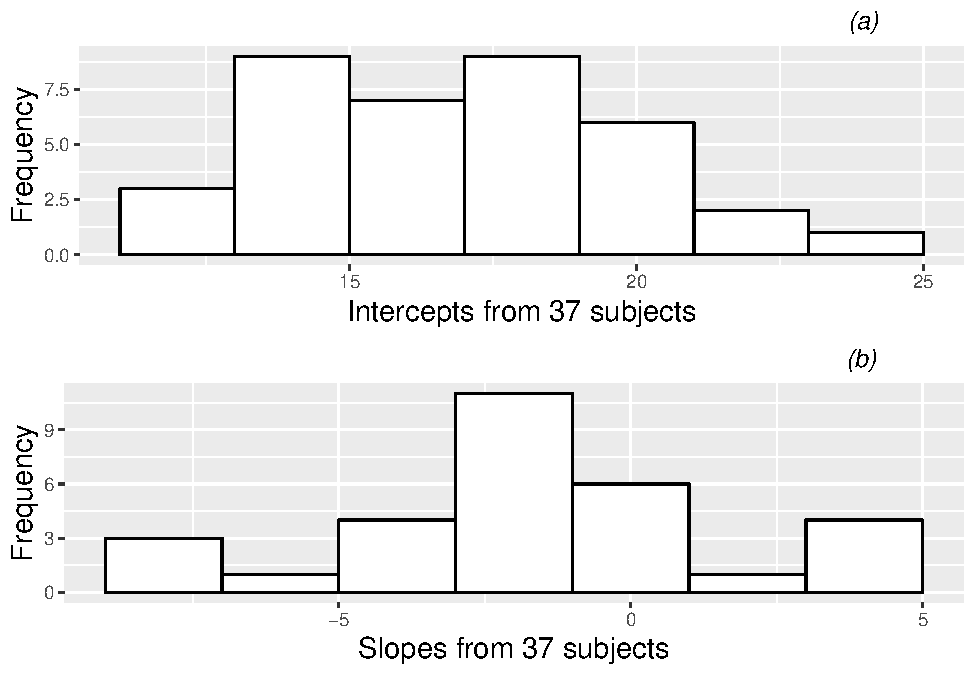
\includegraphics[width=0.6\linewidth]{bookdown-bysh_files/figure-latex/mli-histmat2-1} 

}

\caption{Histograms of intercepts and slopes from fitting simple regression models by subject, where each model contained a single binary predictor indicating if a performance was part of a large ensemble.}\label{fig:mli-histmat2}
\end{figure}

As an illustration, we can consider whether or not there are significant relationships between individual regression parameters (intercepts and slopes) and instrument played. From a modeling perspective, we would build a system of two \textbf{Level Two models} to predict the fitted intercept (\(a_{i}\)) and fitted slopes (\(b_{i}\)) for Subject \(i\):

\begin{align}
a_{i} & =  \alpha_{0}+\alpha_{1}\textstyle{Orch}_{i}+u_{i}
\label{eq:level2s0}  \\
b_{i} & =  \beta_{0}+\beta_{1}\textstyle{Orch}_{i}+v_{i}
\label{eq:level2s1}
\end{align}
where \(\textstyle{Orch}_{i}=1\) if Subject \(i\) plays an orchestral instrument and \(\textstyle{Orch}_{i}=0\) if Subject \(i\) plays keyboard or is a vocalist. Note that, at Level Two, our response variables are not observed measurements such as performance anxiety scores, but rather the fitted regression coefficients from the Level One models fit to each subject. (Well, in our theoretical model, the responses are actually the true intercepts and slopes from Level One models for each subject, but in reality, we have to use our estimated slopes and intercepts.)

Exploratory data analysis (see boxplots by instrument in Figure \ref{fig:mli-boxmat2}) suggests that subjects playing orchestral instruments have higher intercepts than vocalists or keyboardists, and that orchestral instruments are associated with slight lower (more negative) slopes, although with less variability that the slopes of vocalists and keyboardists. These trends are borne out in regression modeling. If we fit Equations \eqref{eq:level2s0} and \eqref{eq:level2s1} using fitted intercepts and slopes as our response variables, we obtain the following estimated parameters: \(\hat{\alpha}_{0}=16.3\), \(\hat{\alpha}_{1}=1.4\), \(\hat{\beta}_{0}=-0.8\), and \(\hat{\beta}_{1}=-1.4\). Thus, the intercept (\(a_{i}\)) and slope (\(b_{i}\)) for Subject \(i\) can be modeled as:

\begin{align}
\hat{a}_{i} & = 16.3+1.4\textstyle{Orch}_{i}+u_{i}
\label{eq:level2s0hat}  \\
\hat{b}_{i} & = -0.8-1.4\textstyle{Orch}_{i}+v_{i}
\label{eq:level2s1hat}
\end{align}
where \(a_{i}\) is the true mean negative affect when Subject \(i\) is playing solos or small ensembles, and \(b_{i}\) is the true mean difference in negative affect for Subject \(i\) between large ensembles and other performance types. Based on these models, average performance anxiety before solos and small ensembles is 16.3 for vocalists and keyboardists, but 17.7 (1.4 points higher) for orchestral instrumentalists. Before playing in large ensembles, vocalists and instrumentalists have performance anxiety (15.5) which is 0.8 points lower, on average, than before solos and small ensembles, while subjects playing orchestral instruments experience an average difference of 2.2 points, producing an average performance anxiety of 15.5 before playing in large ensembles just like subjects playing other instruments. However, the difference between orchestral instruments and others does not appear to be statistically significant for either intercepts (t=1.424, p=0.163) or slopes (t=-1.168, p=0.253).

\begin{figure}

{\centering 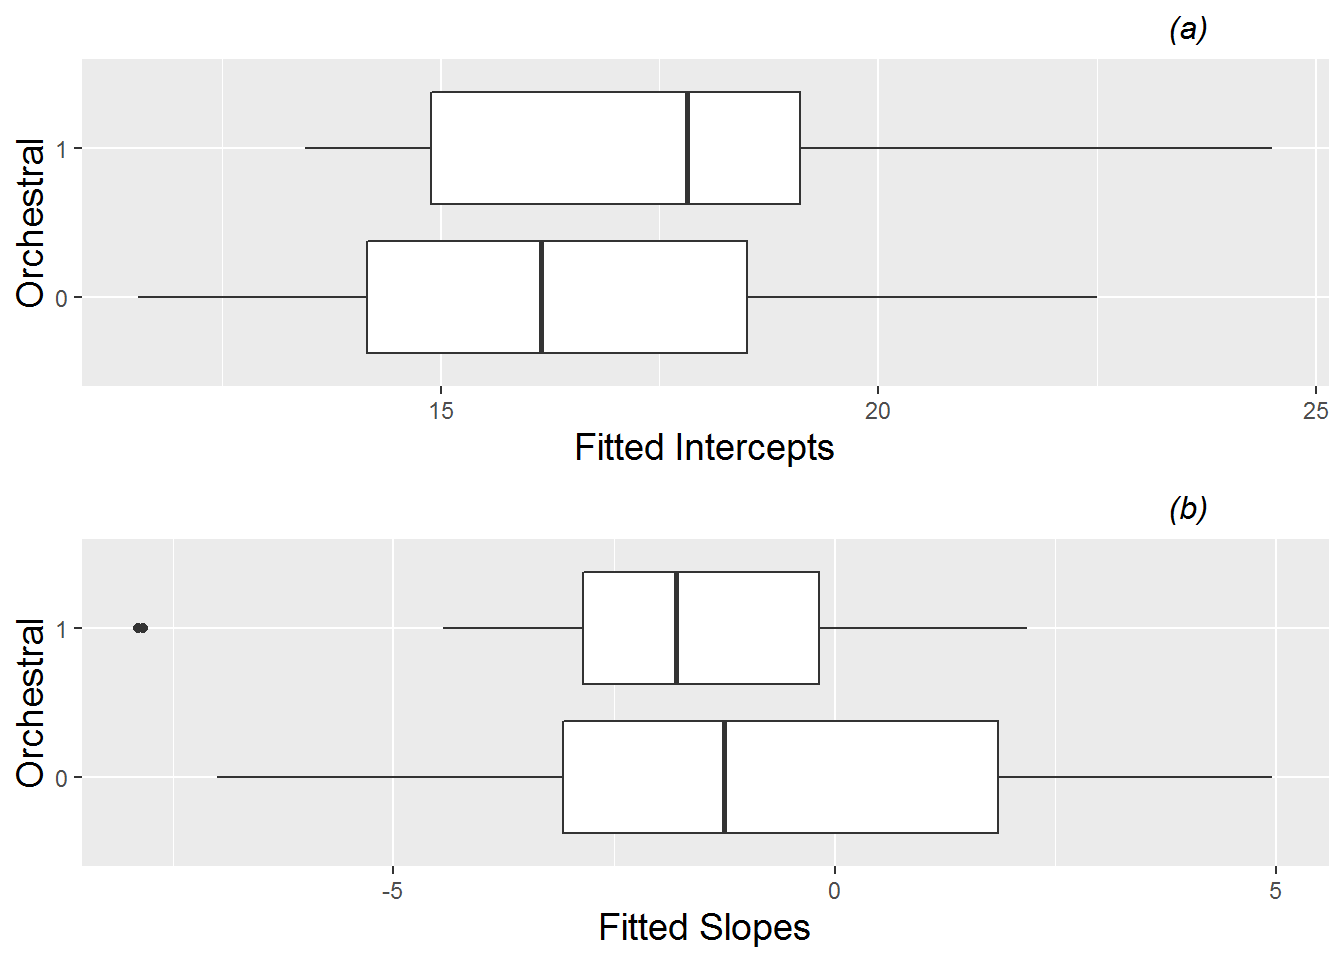
\includegraphics[width=0.6\linewidth]{bookdown-bysh_files/figure-latex/mli-boxmat2-1} 

}

\caption{Boxplots of fitted intercepts (plot (a)) and slopes (plot (b)) by orchestral instrument (1) vs. keyboard or vocalist (0).}\label{fig:mli-boxmat2}
\end{figure}

This two stage modeling process does have some drawbacks. Among other things, (1) it weights every subject the same regardless of the number of diary entries we have, (2) it responds to missing individual slopes (from 7 subjects who never performed in a large ensemble) by simply dropping those subjects, and (3) it does not share strength effectively across individuals. These issues can be better handled through a unified multilevel modeling framework which we will develop over the remainder of this section.

\hypertarget{twolevelmodelingunified}{%
\section{Two level modeling: a unified approach}\label{twolevelmodelingunified}}

\hypertarget{ourframework}{%
\subsection{Our framework}\label{ourframework}}

For the unified approach, we will still envision two levels of models as in section \ref{twostage}, but we will use likelihood-based methods for parameter estimation rather than ordinary least squares to address the drawbacks associated with the two-stage approach. To illustrate the unified approach, we will first generalize the models presented in section \ref{twostage}. Let \(Y_{ij}\) be the performance anxiety score of the \(i^{th}\) subject before performance \(j\). If we are initially interested in examining the effects of playing in a large ensemble and playing an orchestral instrument, then we can model the performance anxiety for Subject \(i\) in performance \(j\) with the following system of equations:

\begin{itemize}
\tightlist
\item
  Level One:
  \begin{equation}
  Y_{ij} = a_{i}+b_{i}\textstyle{LargeEns}_{ij}+\epsilon_{ij}
  \label{eq:level1large}
  \end{equation}
\item
  Level Two:
  \begin{align*}
  a_{i} & = \alpha_{0}+\alpha_{1}\textstyle{Orch}_{i}+u_{i} \\
  b_{i} & = \beta_{0}+\beta_{1}\textstyle{Orch}_{i}+v_{i},
  \end{align*}
\end{itemize}

In this system, there are 4 key \textbf{fixed effects} to estimate: \(\alpha_{0}\), \(\alpha_{1}\), \(\beta_{0}\) and \(\beta_{1}\). Fixed effects are the fixed but unknown population effects associated with certain covariates. The intercepts and slopes for each subject from Level One, \(a_{i}\) and \(b_{i}\), don't need to be formally estimated as we did in section \ref{twostage}; they serve to conceptually connect Level One with Level Two. In fact, by substituting the two Level Two equations into the Level One equation, we can view this two-level system of models as a single \textbf{Composite Model} without \(a_{i}\) and \(b_{i}\):

\begin{align*}
Y_{ij} & = [\alpha_{0}+\alpha_{1}\textstyle{Orch}_{i}+\beta_{0}\textstyle{LargeEns}_{ij}+\beta_{1}\textstyle{Orch}_{i}\textstyle{LargeEns}_{ij}] \\
 & \textrm{} + [u_{i}+v_{i}\textstyle{LargeEns}_{ij}+\epsilon_{ij}]
\end{align*}

From this point forward, when building multilevel models, we will use Greek letters (such as \(\alpha_{0}\)) to denote final fixed effects model parameters to be estimated empirically, and Roman letters (such as \(a_{0}\)) to denote preliminary fixed effects parameters at lower levels. Variance components that will be estimated empirically will be denoted with \(\sigma\) or \(\rho\), while terms such as \(\epsilon\) and \(u_{i}\) represent error terms. In our framework, we can estimate final parameters directly without first estimating preliminary parameters, which can be seen with the Composite Model formulation (although we can obtain estimates of preliminary parameters in those occasional cases when they are of interest to us). Note that when we model a slope term like \(b_{i}\) from Level One using Level Two covariates like \(\textstyle{Orch}_{i}\), the resulting Composite Model contains a \textbf{cross-level interaction term}, denoting that the effect of \(\textstyle{LargeEns}_{ij}\) depends on the instrument played.

Furthermore, with a binary predictor at Level Two such as instrument, we can write out what our Level Two model looks like for those who play keyboard or are vocalists (\(\textstyle{Orch}_{i}=0\)) and those who play orchestral instruments (\(\textstyle{Orch}_{i}=1\)):

\begin{itemize}
\tightlist
\item
  Keyboardists and Vocalists (\(\textstyle{Orch}_{i}=0\))
\end{itemize}

\begin{align*}
a_{i} & = \alpha_{0}+u_{i} \\
b_{i} & = \beta_{0}+v_{i}
\end{align*}
- Orchestral instrumentalists (\(\textstyle{Orch}_{i}=1\))

\begin{align*}
a_{i} & = (\alpha_{0}+\alpha_{1})+u_{i} \\
b_{i} & = (\beta_{0}+\beta_{1})+v_{i}
\label{eq:level2byorch}
\end{align*}

Writing the Level Two model in this manner helps us interpret the model parameters from our two-level model. In this case, even the Level One covariate is binary, so that we can write out expressions for mean performance anxiety based on our model for four different combinations of instrument played and performance type:

\begin{itemize}
\tightlist
\item
  Keyboardists or vocalists playing solos or small ensembles: \(\alpha_{0}\)
\item
  Keyboardists or vocalists playing large ensembles: \(\alpha_{0}+\beta_{0}\)
\item
  Orchestral instrumentalists playing solos or small ensembles: \(\alpha_{0}+\alpha_{1}\)
\item
  Orchestral instrumentalists playing large ensembles: \(\alpha_{0}+\alpha_{1}+\beta_{0}+\beta_{1}\)
\end{itemize}

\hypertarget{random-vs.-fixed-effects}{%
\subsection{Random vs.~fixed effects}\label{random-vs.-fixed-effects}}

Before we can use likelihood-based methods to estimate our model parameters, we still must define the distributions of our error terms. The error terms \(\epsilon_{ij}\), \(u_{i}\), and \(v_{i}\) represent random effects in our model. In multilevel models, it is important to distinguish between fixed and random effects. Typically, \textbf{fixed effects} describe levels of a factor that we are specifically interested in drawing inferences about, and which would not change in replications of the study. For example, in our music performance anxiety case study, the levels of performance type will most likely remain as solos, small ensembles, and large ensembles even in replications of the study, and we wish to draw specific conclusions about differences between these three types of performances. Thus, performance type would be considered a fixed effect. On the other hand, \textbf{random effects} describe levels of a factor which can be thought of as a sample from a larger population of factor levels; we are not typically interested in drawing conclusions about specific levels of a random effect, although we are interested in accounting for the influence of the random effect in our model. For example, in our case study the different musicians included can be thought of as a random sample from a population of performing musicians. Although our goal is not to make specific conclusions about differences between any two musicians, we do want to account for inherent differences among musicians in our model, and by doing so, we will be able to draw more precise conclusions about our fixed effects of interest. Thus, musician would be considered a random effect.

\hypertarget{MVN}{%
\subsection{Distribution of errors: the multivariate normal distribution}\label{MVN}}

As part of our multilevel model, we must provide probability distributions to describe the behavior of random effects. Typically, we assume that random effects follow a normal distribution with mean 0 and a variance parameter which must be estimated from the data. For example, at Level One, we will assume that the errors associated with each performance of a particular musician can be described as: \(\epsilon_{ij}\sim N(0,\sigma^2)\). At Level Two, we have one error term (\(u_{i}\)) associated with subject-to-subject differences in intercepts, and one error term (\(v_{i}\)) associated with subject-to-subject differences in slopes. That is, \(u_{i}\) represents the deviation of Subject \(i\) from the mean performance anxiety before solos and small ensembles after accounting for their instrument, and \(v_{i}\) represents the deviation of Subject \(i\) from the mean difference in performance anxiety between large ensembles and other performance types after accounting for their instrument.

In modeling the random behavior of \(u_{i}\) and \(v_{i}\), we must also account for the possibility that random effects at the same level might be correlated. Subjects with higher baseline performance anxiety have a greater capacity for showing decreased anxiety in large ensembles as compared to solos and small ensembles, so we might expect that subjects with larger intercepts (performance anxiety before solos and small ensembles) would have smaller slopes (indicating greater decreases in anxiety before large ensembles). In fact, our fitted Level One intercepts and slopes in this example actually show evidence of a fairly strong negative correlation (\(r=-0.525\), see Figure \ref{fig:mli-scat1}).

\begin{figure}

{\centering 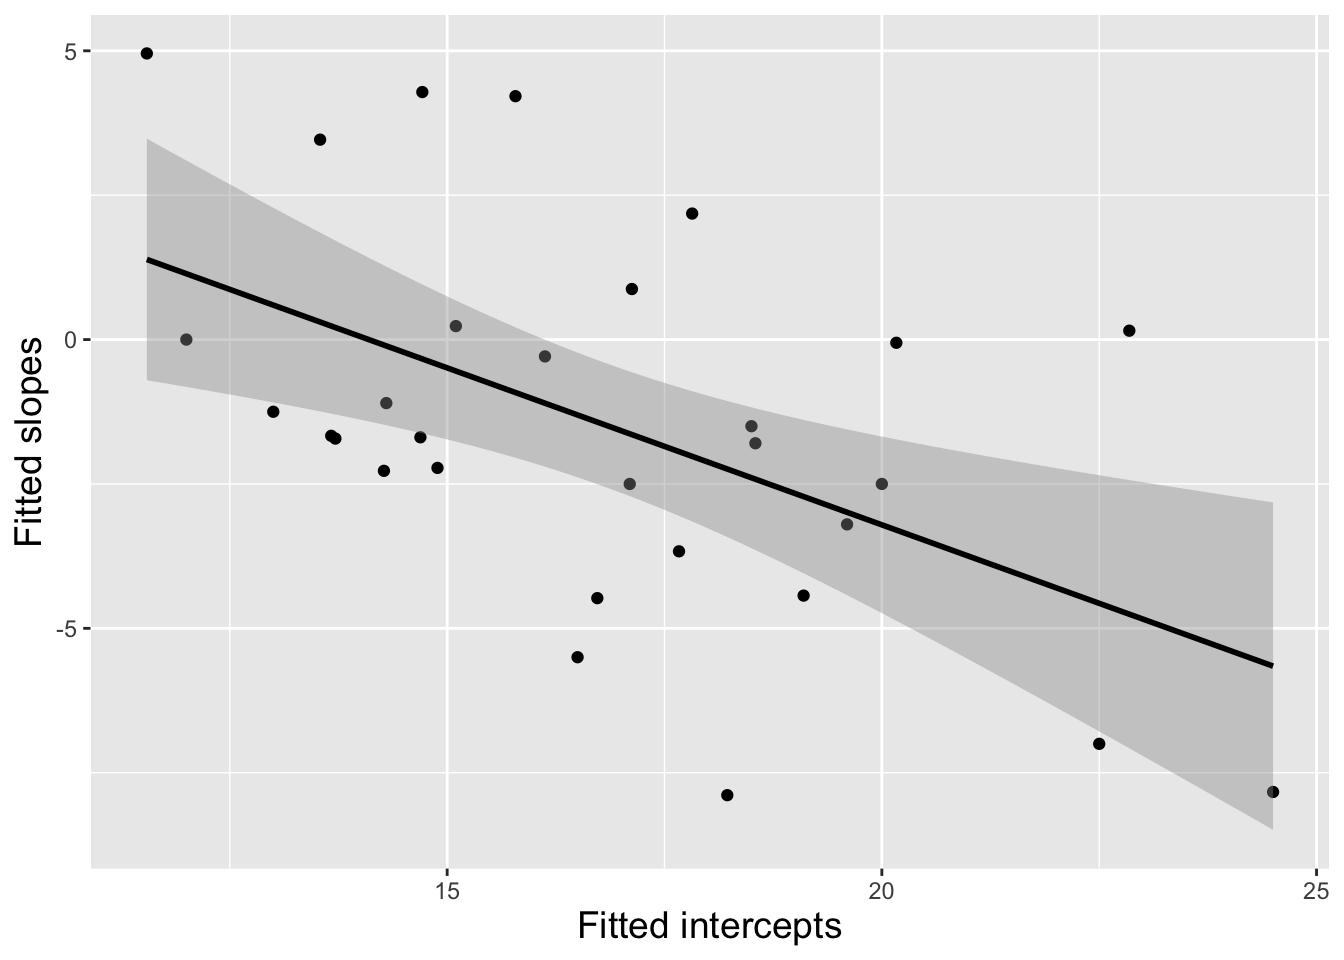
\includegraphics[width=0.6\linewidth]{bookdown-bysh_files/figure-latex/mli-scat1-1} 

}

\caption{Scatterplot with fitted regression line for estimated intercepts and slopes (one point per subject).}\label{fig:mli-scat1}
\end{figure}

To allow for this correlation, the error terms at Level Two can be assumed to follow a multivariate normal distribution in our unified multilevel model. Mathematically, we can express this as:

\begin{equation} 
\left[ \begin{array}{c}
            u_{i} \\ v_{i}
          \end{array}  \right] \sim N \left( \left[
          \begin{array}{c}
            0 \\ 0
          \end{array} \right], \left[
          \begin{array}{cc}
            \sigma_{u}^{2} & \rho_{uv}\sigma_{u}\sigma_v \\
            \rho_{uv}\sigma_{u}\sigma_v & \sigma_{v}^{2}
          \end{array} \right] \right) 
\label{eq:mvnormal}
\end{equation}
where \(\sigma_{u}^{2}\) is the variance of the \(u_{i}\) terms, \(\sigma_{v}^{2}\) is the variance of the \(v_{i}\) terms, and \(\sigma_{uv} = \rho_{uv}\sigma_{u}\sigma_v\) is the covariance between the \(u_{i}\) and the \(v_{i}\) terms (i.e., how those two terms vary together).

Note that the correlation \(\rho_{uv}\) between the error terms is simply the covariance \(\sigma_{uv}=\rho_{uv}\sigma_{u}\sigma_{v}\) converted to a \([-1,1]\) scale through the relationship:

\begin{equation}
\rho_{uv} = \frac{\sigma_{uv}}{\sigma_{u}\sigma_{v}}
\label{eq:cor}
\end{equation}

With this expression, we are allowing each error term to have its own variance (around a mean of 0) and each pair of error terms to have its own covariance (or correlation). Thus, if there are \(n\) equations at Level Two, we can have \(n\) variance terms and \(n(n-1)/2\) covariance terms for a total of \(n + n(n-1)/2\) variance components. These variance components are organized in matrix form, with variance terms along the diagonal and covariance terms in the off-diagonal. In our small example, we have \(n=2\) equations at Level Two, so we have 3 variance components to estimate---2 variance terms (\(\sigma_{u}^{2}\) and \(\sigma_{v}^{2}\)) and 1 correlation (\(\rho_{uv}\)).

The multivariate normal distribution with \(n=2\) is illustrated in Figure \ref{fig:contour-boundary} for two cases: (a) the error terms are uncorrelated (\(\sigma_{uv}=\rho_{uv}=0\)), and (b) the error terms are positively correlated (\(\sigma_{uv}>0\) and \(\rho_{uv} > 0\)). In general, if the errors in intercepts (\(u_{i}\)) are placed on the x-axis and the errors in slopes (\(v_{i}\)) are placed on the y-axis, then \(\sigma_{u}^{2}\) measures spread in the x-direction and \(\sigma_{v}^{2}\) measures spread in the y-direction, while \(\sigma_{uv}\) measures tilt. Positive tilt (\(\sigma_{uv}>0\)) indicates a tendency for errors from the same subject to both be positive or both be negative, while negative tilt (\(\sigma_{uv}<0\)) indicates a tendency for one error from a subject to be positive and the other to be negative. In Figure \ref{fig:contour-boundary}, \(\sigma_{u}^{2}=4\) and \(\sigma_{v}^{2}=1\), so both contour plots show a greater range of errors in the x-direction than the y-direction. Ellipses near the center of the contour plot indicate pairs of \(u_{i}\) and \(v_{i}\) that are more likely. In Figure \ref{fig:contour-boundary} (a) \(\sigma_{uv}=\rho_{uv}=0\), so the axes of the contour plot correspond to the x- and y-axes, but in Figure \ref{fig:contour-boundary} (b) \(\sigma_{uv}=1.5\), so the contour plot tilts up, reflecting a tendency for high values of \(u_{i}\) to be associated with high values of \(v_{i}\).

\begin{figure}

{\centering 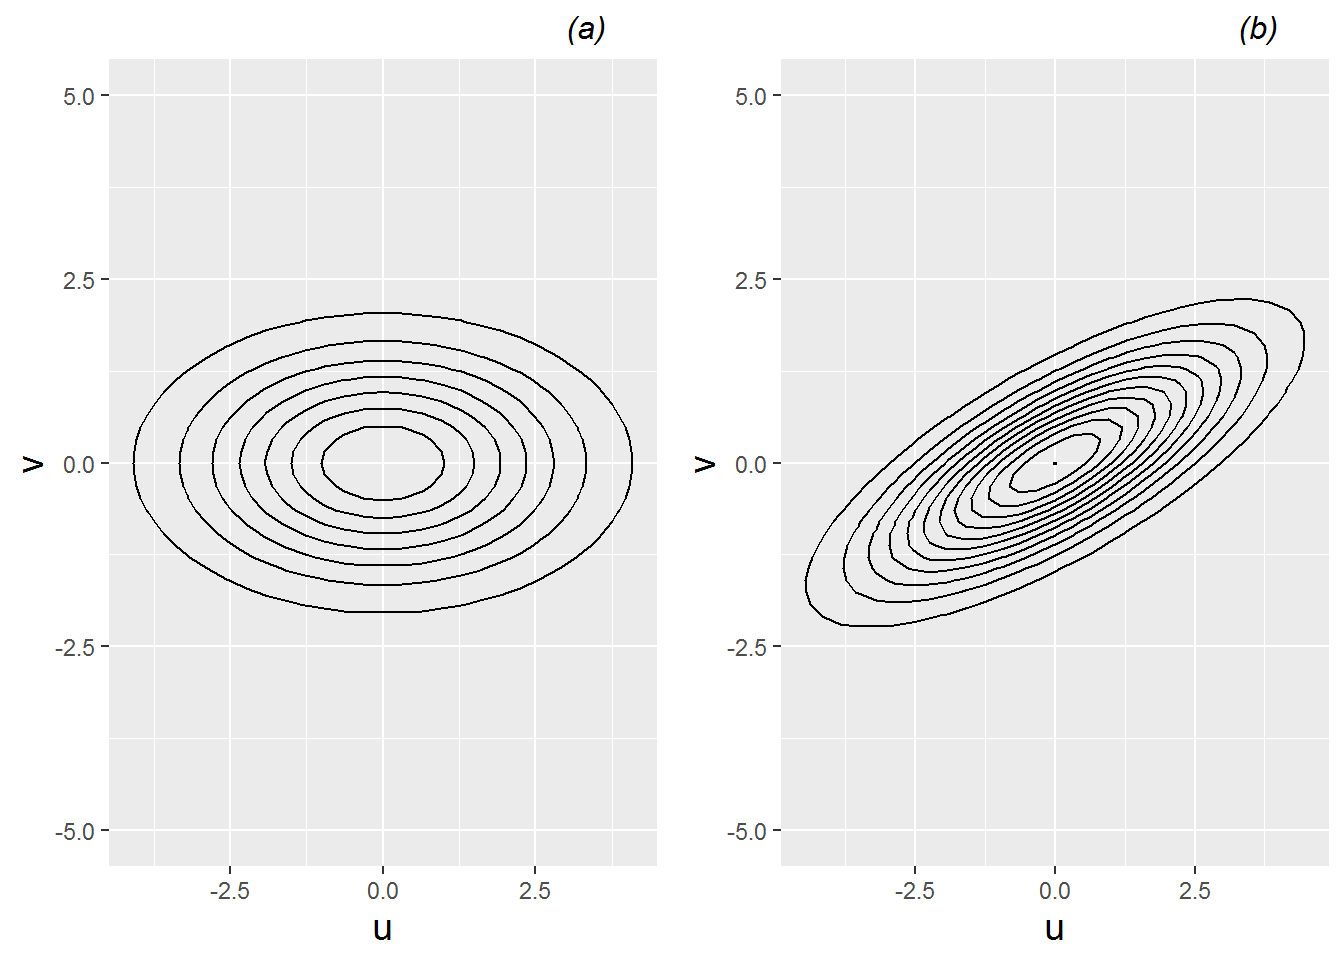
\includegraphics[width=0.6\linewidth]{bookdown-bysh_files/figure-latex/contour-boundary-1} 

}

\caption{Contour plots illustrating a multivariate normal density with (a) no correlation between error terms, and (b) positive correlation between error terms.}\label{fig:contour-boundary}
\end{figure}

\hypertarget{multileveltechnical}{%
\subsection{Technical issues when estimating and testing parameters (Optional)}\label{multileveltechnical}}

Now, our relatively simple two-level model has 8 parameters that need to be estimated: 4 fixed effects (\(\alpha_{0}\), \(\alpha_{1}\), \(\beta_{0}\), and \(\beta_{1}\)), and 4 variance components (\(\sigma^{2}\), \(\sigma_{u}^{2}\), \(\sigma_{v}^{2}\), and \(\sigma_{uv}\)). Note that we use the term \textbf{variance components} to signify model parameters that describe the behavior of random effects. We can use statistical software, such as the lmer() function from the lme4 package in R, to obtain parameter estimates using our 497 observations. The most common methods for estimating model parameters---both fixed effects and variance components---are maximum likelihood (ML) and restricted maximum likelihood (REML). The method of maximum likelihood (ML) was introduced in Chapter \ref{ch-beyondmost}, where parameter estimates are chosen to maximize the value of the likelihood function based on observed data. Restricted maximum likelihood (REML) is conditional on the fixed effects, so that the part of the data used for estimating variance components is separated from that used for estimating fixed effects. Thus REML, by accounting for the loss in degrees of freedom from estimating the fixed effects, provides an unbiased estimate of variance components, while ML estimators for variance components are biased under assumptions of normality, since they use estimated fixed effects rather than the true values. REML is preferable when the number of parameters is large or the primary interest is obtaining estimates of model parameters, either fixed effects or variance components associated with random effects. ML should be used if nested fixed effects models are being compared using a likelihood ratio test, although REML is fine for nested models of random effects (with the same fixed effects model). In this text, we will typically report REML estimates unless we are specifically comparing nested models with the same random effects. In most case studies and most models we consider, there is very little difference between ML and REML parameter estimates. Additional details are beyond the scope of this book \citep{Singer2003}.

Note that the multilevel output shown beginning in the next section contains no p-values for performing hypothesis tests. This is primarily because the exact distribution of the test statistics under the null hypothesis (no fixed effect) is unknown, primarily because the exact degrees of freedom is not known \citep{Bates2015}. Finding good approximate distributions for test statistics (and thus good approximate p-values) in multilevel models is an area of active research. In most cases, we can simply conclude that t-values (ratios of parameter estimates to estimated standard errors) with absolute value above 2 indicate significant evidence that a particular model parameter is different than 0. Certain software packages will report p-values corresponding to hypothesis tests for parameters of fixed effects; these packages are typically using conservative assumptions, large-sample results, or approximate degrees of freedom for a t-distribution. In section \ref{multreg-boot}, we introduced the bootstrap as a non-parametric, computational approach for producing confidence intervals for model parameters. In addition, in section \ref{threelevel-paraboot}, we will introduce a method called the parametric bootstrap which is being used more frequently by researchers to better approximate the distribution of the likelihood test statistic and produce more accurate p-values by simulating data under the null hypothesis \citep{Efron2012}.

\hypertarget{initialmodel}{%
\subsection{An initial model with parameter interpretations}\label{initialmodel}}

The output below contains likelihood-based estimates of our 8 parameters from a two-level model applied to the music performance anxiety data:

\begin{verbatim}
    Linear mixed model fit by REML ['lmerMod'] 
 A)  Formula: na ~ orch + large + orch:large + (large | id) 
        Data: music 
 B)  REML criterion at convergence: 2987 
      
 B2)      AIC      BIC   logLik deviance df.resid  
         3007     3041    -1496     2991      489  
      
     Random effects: 
      Groups   Name        Variance Std.Dev. Corr  
 C)   id       (Intercept)  5.655   2.378          
 D)            large        0.452   0.672    -0.63 
 E)   Residual             21.807   4.670          
 F)  Number of obs: 497, groups:  id, 37 
      
     Fixed effects: 
                 Estimate Std. Error t value 
 G)  (Intercept)   15.930      0.641   24.83 
 H)  orch           1.693      0.945    1.79 
 I)  large         -0.911      0.845   -1.08 
 J)  orch:large    -1.424      1.099   -1.30
\end{verbatim}

This output (except for the capital letters along the left column) was specifically generated by the lmer() function in R; multilevel modeling results from other packages will contain similar elements. Because we will use lmer() output to summarize analyses of case studies in this and following sections, we will spend a little time now orienting ourselves to the most important features in this output.

\begin{itemize}
\tightlist
\item
  A: How our multilevel model is written in R, based on the composite model formulation. For more details, see section \ref{notesr8}.
\item
  B: Measures of model performance. Since this model was fit using REML, this line only contains the REML criterion.
\item
  B2: If the model is fit with ML instead of REML, the measures of performance will contain AIC, BIC, deviance, and the log-likelihood.
\item
  C: Estimated variance components (\(\hat{\sigma}_{u}^2\) and \(\hat{\sigma}_{u}\)) associated with the intercept equation in Level Two.
\item
  D: Estimated variance components (\(\hat{\sigma}_{v}^2\) and \(\hat{\sigma}_{v}\)) associated with the large ensemble effect equation in Level Two, along with the estimated correlation (\(\hat{\rho}_{uv}\)) between the two Level Two error terms.
\item
  E: Estimated variance components (\(\hat{\sigma}^2\) and \(\hat{\sigma}\)) associated with the Level One equation.
\item
  F: Total number of performances where data was collected (Level One observations = 497) and total number of subjects (Level Two observations = 37).
\item
  G: Estimated fixed effect (\(\hat{\alpha}_{0}\)) for the intercept term, along with its standard error and t-value (which is the ratio of the estimated coefficient to its standard error). As described in section \ref{multileveltechnical}, no p-value testing the significance of the coefficient is provided because the exact null distribution of the t-value is unknown.
\item
  H: Estimated fixed effect (\(\hat{\alpha}_{1}\)) for the orchestral instrument effect, along with its standard error and t-value .
\item
  I: Estimated fixed effect (\(\hat{\beta}_{0}\)) for the large ensemble effect, along with its standard error and t-value.
\item
  J: Estimated fixed effect (\(\hat{\beta}_{1}\)) for the interaction between orchestral instruments and large ensembles, along with its standard error and t-value.
\end{itemize}

Assuming the 37 musicians in this study are representative of a larger population of musicians, parameter interpretations for our 8 model parameters are given below:

\begin{itemize}
\tightlist
\item
  Fixed effects:

  \begin{itemize}
  \tightlist
  \item
    \(\hat{\alpha}_{0} = 15.9\). The estimated mean performance anxiety for solos and small ensembles (Large=0) for keyboard players and vocalists (Orch=0) is 15.9.
  \item
    \(\hat{\alpha}_{1} = 1.7\). Orchestral instrumentalists have an estimated mean performance anxiety for solos and small ensembles which is 1.7 points higher than keyboard players and vocalists.
  \item
    \(\hat{\beta}_{0} = -0.9\). Keyboard players and vocalists have an estimated mean decrease in performance anxiety of 0.9 points when playing in large ensembles instead of solos or small ensembles.
  \item
    \(\hat{\beta}_{1} = -1.4\). Orchestral instrumentalists have an estimated mean decrease in performance anxiety of 2.3 points when playing in large ensembles instead of solos or small ensembles, 1.4 points greater than the mean decrease among keyboard players and vocalists.
  \end{itemize}
\item
  Variance components

  \begin{itemize}
  \tightlist
  \item
    \(\hat{\sigma}_{u} = 2.4\). The estimated standard deviation of performance anxiety levels for solos and small ensembles is 2.4 points, after controlling for instrument played.
  \item
    \(\hat{\sigma}_{v} = 0.7\). The estimated standard deviation of differences in performance anxiety levels between large ensembles and other performance types is 0.7 points, after controlling for instrument played.
  \item
    \(\hat{\rho}_{uv} = -0.64\). The estimated correlation between performance anxiety scores for solos and small ensembles and increases in performance anxiety for large ensembles is -0.64, after controlling for instrument played. Those subjects with higher performance anxiety scores for solos and small ensembles tend to have greater decreases in performance anxiety for large ensemble performances.
  \item
    \(\hat{\sigma} = 4.7.\) The estimated standard deviation in residuals for the individual regression models is 4.7 points.
  \end{itemize}
\end{itemize}

Table \ref{tab:table3chp8} shows a side-by-side comparison of estimated coefficients from the approaches described to this point. Underlying assumptions, especially regarding the error and correlation structure, differ, and differences in estimated effects are potentially meaningful. Note that some standard errors are greatly \emph{underestimated} under independence, and that no Level One covariates (such as performance type) can be analyzed under a method such as last-visit-carried-forward which uses one observation per subject. Moving forward, we will employ the unified multilevel approach to maximize the information being used to estimate model parameters and to remain faithful to the structure of the data.

\begin{table}

\caption{\label{tab:table3chp8}Comparison of estimated coefficients and standard errors from the approaches mentioned in this section.}
\centering
\begin{tabular}[t]{lllll}
\toprule
Variable & Independence & TwoStage & LVCF & Multilevel\\
\midrule
Intercept & 15.72(0.36) & 16.28(0.67) & 15.20(1.25) & 15.93(0.64)\\
Orch & 1.79(0.55) & 1.41(0.99) & 1.45(1.84) & 1.69(0.95)\\
Large & -0.28(0.79) & -0.77(0.85) & - & -0.91(0.85)\\
Orch*Large & -1.71(1.06) & -1.41(1.20) & - & -1.42(1.10)\\
\bottomrule
\end{tabular}
\end{table}

Two level modeling as done with the music performance anxiety data usually involves fitting a number of models. Subsequent sections will describe a process of starting with the simplest two-level models and building toward a final model which addresses the research questions of interest.

\hypertarget{sec:buildmodel}{%
\section{Building a multilevel model}\label{sec:buildmodel}}

\hypertarget{buildstrategy}{%
\subsection{Model building strategy}\label{buildstrategy}}

Initially, it is advisable to first fit some simple, preliminary models, in part to establish a baseline for evaluating larger models. Then, we can build toward a final model for description and inference by attempting to add important covariates, centering certain variables, and checking model assumptions. In this study, we are particularly interested in Level Two covariates---those subject-specific variables that provide insight into why individuals react differently in anxiety-inducing situations. To get more precise estimates of the effect of Level Two covariates, we also want to control for Level One covariates that describe differences in individual performances.

Our strategy for building multilevel models will begin with extensive exploratory data analysis at each level. Then, after examining models with no predictors to assess variability at each level, we will first focus on creating a Level One model, starting simple and adding terms as necessary. Next, we will move to Level Two models, again starting simple and adding terms as necessary, beginning with the equation for the intercept term. Finally, we will examine the random effects and variance components, beginning with a full set of error terms and then removing covariance terms and variance terms where advisable (for instance, when parameter estimates are failing to converge or producing impossible or unlikely values). This strategy follows closely with that described by \citet{Bryk2002} and used by \citet{Singer2003}. Singer and Willett further find that the modeled error structure rarely matters in practical contexts. Other model building approaches are certainly possible. \citet{Diggle2002}, for example, begins with a saturated fixed effects model, determines variance components based on that, and then simplifies the fixed part of the model after fixing the random part.

\hypertarget{modela}{%
\subsection{An initial model: unconditional means or random intercepts}\label{modela}}

The first model fit in almost any multilevel context should be the \textbf{unconditional means model}, also called a \textbf{random intercepts model}. In this model, there are no predictors at either level; rather, the purpose of the unconditional means model is to assess the amount of variation at each level---to compare variability within subject to variability between subjects. Expanded models will then attempt to explain sources of between and within subject variability.

The unconditional means (random intercepts) model, which we will denote as Model A, can be specified either using formulations at both levels:

\begin{itemize}
\tightlist
\item
  Level One:
  \begin{equation}
  Y_{ij} = a_{i}+\epsilon_{ij} \textrm{ where } \epsilon_{ij}\sim N(0,\sigma^2)
  \label{eq:level1uncmean}
  \end{equation}
\item
  Level Two:
  \begin{equation}
  a_{i} = \alpha_{0}+u_{i} \textrm{ where } u_{i}\sim N(0,\sigma_{u}^{2})
  \label{eq:level2uncmean}
  \end{equation}
\end{itemize}

or as a composite model:
\begin{equation}
Y_{ij}=\alpha_{0}+u_{i}+\epsilon_{ij}
\label{eq:compuncmean}
\end{equation}
In this model, the performance anxiety scores of subject \(i\) are not a function of performance type or any other Level One covariate, so that \(a_{i}\) is the true mean response of all observations for subject \(i\). On the other hand, \(\alpha_{0}\) is the grand mean -- the true mean of all observations across the entire population. Our primary interest in the unconditional means model is the variance components -- \(\sigma^2\) is the within-person variability, while \(\sigma_{u}^{2}\) is the between-person variability. The name \textbf{random intercepts model} then arises from the Level Two equation for \(a_{i}\): each subject's intercept is assumed to be a random value from a normal distribution centered at \(\alpha_{0}\) with variance \(\sigma_{u}^{2}\).

Using the composite model specification, the unconditional means model can be fit to the music performance anxiety data using statistical software:

\begin{Shaded}
\begin{Highlighting}[]
\CommentTok{#Model A (Unconditional means model)}
\NormalTok{model.a <-}\StringTok{ }\KeywordTok{lmer}\NormalTok{(na }\OperatorTok{~}\StringTok{ }\DecValTok{1} \OperatorTok{+}\StringTok{ }\NormalTok{(}\DecValTok{1} \OperatorTok{|}\StringTok{ }\NormalTok{id), }\DataTypeTok{REML =}\NormalTok{ T, }\DataTypeTok{data =}\NormalTok{ music)}
\end{Highlighting}
\end{Shaded}

\begin{verbatim}
##  Groups   Name        Variance Std.Dev.
##  id       (Intercept)  4.95    2.22    
##  Residual             22.46    4.74
\end{verbatim}

\begin{verbatim}
##  Number of Level Two groups =  37
\end{verbatim}

\begin{verbatim}
##             Estimate Std. Error t value
## (Intercept)    16.24     0.4279   37.94
\end{verbatim}

From this output, we obtain estimates of our three model parameters:

\begin{itemize}
\tightlist
\item
  \(\hat{\alpha}_{0}=16.2=\) the estimated mean performance anxiety score across all performances and all subjects.
\item
  \(\hat{\sigma}^2=22.5=\) the estimated variance in within-person deviations.
\item
  \(\hat{\sigma}_{u}^{2}=5.0=\) the estimated variance in between-person deviations.
\end{itemize}

The relative levels of between- and within-person variabilities can be compared through the \textbf{intraclass correlation coefficient}:

\begin{equation}
\hat{\rho}=\frac{\textrm{Between-person variability}}{\textrm{Total variability}} = \frac{\hat{\sigma}_{u}^{2}}{\hat{\sigma}_{u}^{2}+\hat{\sigma}^2} = \frac{5.0}{5.0+22.5} = .182.
\label{eq:intracc}
\end{equation}
Thus, 18.2\% of the total variability in performance anxiety scores are attributable to differences among subjects. In this particular model, we can also say that the average correlation for any pair of responses from the same individual is a moderately low .182. As \(\rho\) approaches 0, responses from an individual are essentially independent and accounting for the multilevel structure of the data becomes less crucial. However, as \(\rho\) approaches 1, repeated observations from the same individual essentially provide no additional information and accounting for the multilevel structure becomes very important. With \(\rho\) near 0, the \textbf{effective sample size} (the number of independent pieces of information we have for modeling) approaches the total number of observations, while with \(\rho\) near 1, the effective sample size approaches the number of subjects in the study.

  \bibliography{bib/articles.bib,bib/books.bib,bib/misc.bib}

\backmatter
\printindex

\end{document}
